\documentclass[a4paper]{article}
\usepackage{lscape}
\usepackage{graphicx}
\usepackage[export]{adjustbox}

%% Language and font encodings
\usepackage[english]{babel}
\usepackage[utf8x]{inputenc}
\usepackage[T1]{fontenc}
\usepackage{makecell}
\usepackage{dblfloatfix}
\usepackage{placeins}

%% Sets page size and margins
\usepackage[a4paper,top=1.7cm,bottom=2cm,left=2cm,right=2cm,marginparwidth=1.75cm]{geometry}

%% Useful packages
\usepackage{amsmath}
\usepackage{graphicx}
\usepackage[colorinlistoftodos]{todonotes}
\usepackage[colorlinks=true, allcolors=blue]{hyperref}
\usepackage{float}
\usepackage{pgfplots}
\usepackage{multirow}
\usepackage{placeins}

\begin{document}
\begin{titlepage}
\centering

\includegraphics[width=0.4\textwidth]{../img/uni.png}\par\vspace{1cm}
	{\scshape\LARGE University of New South Wales \par}
	\vspace{1cm}
	{\huge\bfseries Applying Artificial Intelligence to analyse Retinal Degeneration\par}
	\vspace{2cm}
    \begin{table}[!h]
    \centering
    \begin{tabular}{||c c||} 
    \hline
    
    \large{\textbf{Name}} & \large{\textbf{zID}} \\ [0.5ex] 
    \hline\hline
    \large{Mohamed Daniel Al Mouiee} &\large{z5114185}\\ 
    \hline
    \end{tabular}
    \end{table}

    \vspace{5cm}
    \textbf{Keywords:} \\
    Retinal Degeneration, Artificial Intelligence, Image Classification
    \vspace{2cm}
    
	\vfill

% Bottom of the page
	{\large \today\par}
\end{titlepage}

\newpage
\tableofcontents
\newpage
\listoffigures
\listoftables
\vfill

\newpage

\section{Abbreviations}
\begin{itemize}
    \vspace{3mm}
    \item \textbf{AI}: Artificial Intelligence
    \vspace{3mm}
    \item \textbf{ATP}: Adenosine Tri-Phosphate
    \vspace{3mm}
    \item \textbf{CNN}: Convolutional Neural Network
    \vspace{3mm}
    \item \textbf{FN}: False Negative
    \vspace{3mm}
    \item \textbf{FP}: False Positive
    \vspace{3mm}
    \item \textbf{H\&E}: Haematoxylin and Eosin
    \vspace{3mm}
    \item \textbf{OCT}: Optical Coherence Tomography
    \vspace{3mm}
    \item \textbf{ReLU}: Rectified Linear Unit
    \vspace{3mm}
    \item \textbf{TN}: True Negative
    \vspace{3mm}
    \item \textbf{TP}: True Positive
\end{itemize}

\newpage

\section{Introduction}
The human retina has mystified researchers historically, ever since the development of advanced tools and technologies. This highly specialised tissue is one of great detail, organisation and of high importance to one of our many essential senses, vision \cite{RN1}. Many significant discoveries have been made due to technological advancements which have allowed researchers to investigate this structure. With this exponential growth of technology, it would be of great interest to science and humanity that these technologies be utilised to make further inroads into the area of Retinal research. \vspace{3mm}

Most recently, Artificial Intelligence, and more specifically Deep Learning, has gained great importance in the medical field. It has displayed very encouraging results in image classification tasks for everyday applications such as facial recognition of pedestrians crossing the road \cite{RN3}. Medical researchers have tried to adapt these techniques in many areas of medicine that have challenged them to the extreme. Numerous studies have been conducted using AI to observe the behaviour and characteristics of the retina, for example, Google's research into Diabetic Retinopathy using retinal fundus photographs \cite{RN6}. This showed great results using AI technology, displaying high accuracy results by segregating diseased retinae images from those that are not. The success of artificial intelligence is evident in these cases and there is general optimism that it can be implemented in further medicinal studies.\vspace{3mm}

Despite these studies, a key structure of the retina which has not been analysed rigorously in an AI application is its highly specialised cellular layers. Discoveries have been made which depict the role of certain cells in the retina \cite{RN4}. However, once it begins to degenerate, the role and behaviour of these sections tend to be ambiguous. Many tedious sub tasks in medical research are also a challenge for experts, in addition to simulations not being at the same high standards as other biomedical fields \cite{RN5}. Large amounts of data that detail various levels of retinal damage are available at present, but are not being analysed in an efficient manner. Hence, AI has the potential to make new discoveries regarding the behaviour of retinal degeneration stages.\vspace{3mm}

This project aims to tie the two fields together in attempt to automate the classification of retinal degeneration. This will include the development of a Convolutional Neural Network capable of classifying histologically-stained, retinal images according to the amount of degeneration and the evaluation of its performance for future clinical applications. This ambition matches the optimism that a valuable tool may come about of this research. Ultimately, understanding the way a retina degenerates on a cellular level will give researchers a new perspective into it as well as provide key information to help improve ophthalmological technology, for example the bionic eye \cite{RN24}.
\pagebreak

\section{Literature Review}

    \subsection{Literature and Publication Analysis}
        This project is somewhat open-ended in terms of the type of results we are searching for. The potential which artificial intelligence possesses is great and it has shown extraordinary results that were a mere imagination not too long ago. The application of artificial intelligence in medicine has been debated over the years in terms of its performance and future potential, in addition to ethical issues that explore when and how human interaction is affected. The uniqueness of medicine as a field of study is a difficult factor to manage logistically, as dealing with real-life patients and life-threatening issues has its toll on all participants. Despite the level of advancement we have reached, many aspects are still considerable challenges that must be dealt with in an effective manner.
        \vspace{3mm}

        \subsubsection{Retinal Degeneration}

        Practical solutions for blindness and vision loss have not been developed as of today. Analysing the degenerative process of the retina was almost impossible before the innovation of imaging technologies such as fundus photography, optical coherence tomography and scanning of histologically stained segments of the retina. The more interesting case that can be discussed is the usage of Haematoxylin and Eosin staining of the retinal cellular layers. Marc et al. \cite{RN8} demonstrated that these cellular layers are prone to modifications during the degenerative process of the retina. The process goes through different stages of death and re-circuiting, particularly, within the layers responsible for vision processing such as the photoreceptor cells (rods and cones). Although it states that various stages are observed throughout this process, it is reluctant to conclude that these stages represent a sound classification model for retinal damage. Rather, it can be viewed as a high-level abstraction of the damage which can provide context around the nature of the retina's health. For example, the first stage that can be observed, according to Marc et al., is the degeneration of rods in the Outer Nuclear Layer. It is clear that rods are dying in this stage and can be see in histological images, however, this is on a cellular level only and cannot necessarily be extended to a general "blindness" categorisation. Similarly, the sequential stages of cone degeneration and the migration of particular cells, such as Muller cells to the Inner Nuclear Layer, are not concrete evidence of this classification system being effective. The lack of "blindness" quantification as well as decisive criteria of damage signs are major factors that prompt our application of Artificial Intelligence in retinal analysis.
        \vspace{3mm}

        Further, other researches have reached a similar conclusion in terms of anatomical modifications the retina endures during degeneration. Bloch et al. \cite{RN10} demonstrated that retinitis pigmentosa can be characterised using similar stages, which is shown in the Figure below:
        \vspace{3mm}

        \begin{figure}[h!]
            \centerline{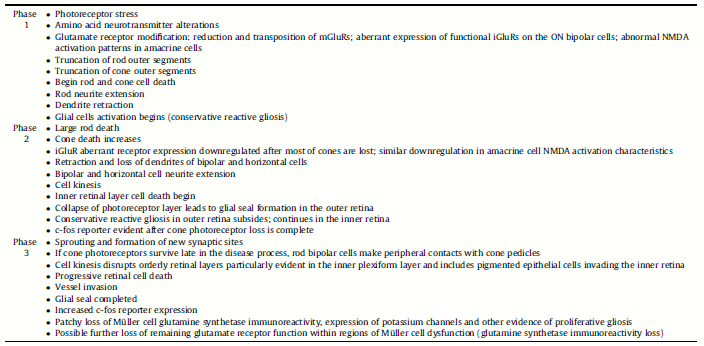
\includegraphics[width=1\textwidth]{../img/damageStages.png}}
            \label{fig 1: Retinal Anatomical Modification} 
        \end{figure}
        \label{fig1:}Stages of retinal anatomical modifications during Retinitis Pigmentosa (Modified after Kalloniatis et al.\cite{RN9})
        \vspace{3mm}
 
        Despite this conformity, it too clearly lacks the confidence in drawing correlations between cellular damage and the quantification of blindness and the vision degeneration process. The difficulty stems from the fact that anatomical changes have not been analysed thoroughly and require intense deconstruction in determining patterns observed in retinal data. Many attempts to reverse this damage have failed and resulted in efforts to bypass natural vision methods for vision-deficient patients, for instance, the implantation of bionic eyes \cite{RN24}. Promising results have been established using this technology where previously blind patients are now able to identify intensities of light as well as patches of black and white objects. These prostheses are still in development and require much more refinement to reach a high level of vision restoration, but early suggestions of it being an optimal alternative to irreversible damage to the retina are promising. As along as the optic nerve that connects to the retina is healthy, it can be utilised in these effective solutions.
        \vspace{3mm}

        Currently, researchers are in the pursuit of how the retina specifically behaves as degeneration takes it toll on it. Establishing this key relationship between retina functionality and vision performance is vital in optimising these prostheses. As discussed in the paper by Bloch et al. \cite{RN10}, many of the implants succeeded in producing artificial vision but are subjected to many limitations as opposed to natural vision. Establishing the link that increases the quality of artificial vision will help boost the effectiveness of these devices, thus increasing the quality of life for these patients. Bloch et al. \cite{RN10} understood that many of the current systems that are in place for artificial vision do not have a clear advantage over the rest, mentioning the need for a clear and concise standard for blindness quantification. Unifying this will assist future studies in managing the approach taken to analyse the aforementioned relationship. They did, however, fall short of mentioning the need for better analysis of histological retinal examinations. Attempting to relate the enigma of blindness stages, with the help of H\&E high resolution images, to retinal damage will certainly assist in making inroads towards this objective.
        \vspace{3mm}

        Many researchers have acknowledged the power of histological data and its potential to uncover hidden information about structures and functionalities. A strong advocate of this is the research on images of breast cancer cells stained with H\&E by Zheng et al. \cite{RN13}. This is probably the closest study to what will be performed in this project in regards to H\&E automated classification. Zheng et al. demonstrated not only the potential of histological data, but also the power of artificial intelligence, more specifically Convolutional Neural Networks. This type of images is very useful in detailing structures accurately and in a well defined manner. 'Well-defined' can be interpreted here as the ability to concisely distinguish between heterogenous structures as well as identify the differences between homogenous structures. In Zheng et al's case, this is the determination of which component in the image represents the nucleus (heterogenous structure distinction), in addition to analysing physical characteristics when considering whether an image is of a malignant or benign tumour (homogenous structure differences). While this may seem like the daily task of an oncologist, the accuracy at which this artificially intelligent system determined the nature of breast cancer tumours was excitingly high. This non-specialist machine, which does not have years of histological data analysis training, demonstrated exciting results which took a fraction of the resources used to train an oncologist. Zheng et al's model achieved levels of accuracy that may well compete with those of an experienced professional. The model was able to distinguish between 2 classes of images consisting of malignant and benign tumours with high levels of accuracy. The below table shows the results for this 2-class model:
        \vspace{3mm}

        \begin{table}[!h]
            \centering
                \begin{tabular}{||c c c||} 
                \hline
                \textbf{Sensitivity (\%)} & \textbf{Specificity (\%)} & \textbf{Accuracy (\%)} \\ 
                \hline\hline
                0.955 & 0.964  & \textbf{0.959} \\
                \hline
                \end{tabular}
            \caption{\label{fig:2} Accuracy values for Zheng et al. 2-class model}
        \end{table}

        In addition to this model, a more interesting 15-class network was also developed demonstrating, once more, high levels of accuracy. The network did utilise the nucleus within cells to assist with spatial calculations and determining the output, but what could have helped the network to excel was the use of annotations. By annotating specific structures and layers within a cell the model could have easily identified similar structures it has seen previously and formulate new discoveries about patterns within damaged cells. The potential of H\&E analysis is not to be underestimated and there must be further studies devoted to uncovering the hidden patterns that might hold the key to new discoveries. The proposed RetinaNET solution in this paper hopes to utilise this data effectively and make progress towards areas of retinal data management.
        \vspace{3mm}

        Although previous histological automated analysis has been carried out on different anatomical structures, it is worth noting that retinal histology has not had its fair share. No publication, to this date, has investigated the use of artificial intelligence on retinal H\&E stained images. This project will attempt to bridge this gap in literature where the application of Convolutional Neural Networks on this type of medical images for the retina will make progress towards demystifying it. Having stated this, there are a number of researches into other types of retina images using artificial intelligence and have developed feasible solutions that may be commercialised sometime in the future.
        \vspace{3mm}

        Google incorporated has taken big steps in this field where Gulshan et al. \cite{RN6} made use of millions of retinal fundus photographs that are available in abundance from eye clinics, hospitals and research facilities. The study was conducted to determine whether an artificially intelligent algorithm can be produced to detect the presence of \textit{Diabetic Retinopathy} and \textit{Diabetic Macular Edema} in these images. The brilliance that lays hidden within these models is the ability to learn without specifying set rules as Gulshan et al. \cite{RN6} state. To ensure that the model' performance is verified, the images are graded by variously experienced ophthalmologists giving a large range of assessments for similar images of diseased retinae. In addition to the verification, the dataset is noticeably large enough to produce interesting results had the system been designed for many different classes. This is a common issue in artificial intelligence as obtaining large quantities of certain data may prove to be the hardest step even before developing solutions. In this project, the datasets of H\&E stained retina of felines were obtained as part of a project at UNSW, as these types of images are not largely available to the public or researchers. As a result of this scarcity, the size of this dataset is small in comparison to many deep learning projects. Gulshan et al. \cite{RN6} managed to use over 120000 images for development which is an important factor that contributed to the model's success (mean sensitivity and specificity of 97.5\% and 93.4\% respectively).
        \vspace{3mm}

        The analysis of retinal data using AI can also be used to determine other health factors not relating to vision. An example of this is the study of Poplin et al. where cardiovascular risk factors are predicted using retinal fundus photographs \cite{RN15}. Structures located in the eye and retina provide information that can be related to cardiovascular disease relevance. Predicted values included systolic blood pressure (SBP) and life expectancy of participants who undertook digital screening of their retinae. The results were interesting as the mean absolute error for there 2 factors were relatively low (11.23 mmHG and 3.26 years respectively). Once again, this is strong evidence of the potential application of automated retinal analysis, however the results did display a reoccurring pattern. This is illustrated in plot below obtained from Poplin et al.:
        \vspace{3mm}

        \begin{figure}[h!]
            \centerline{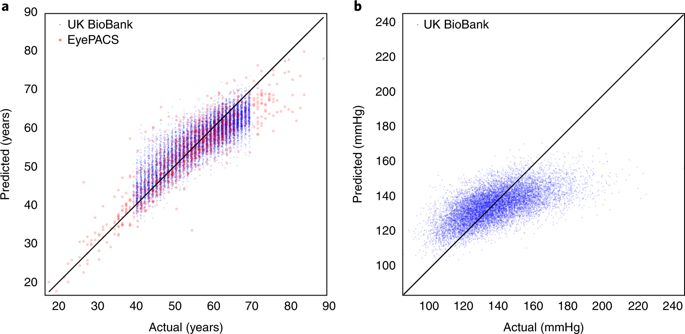
\includegraphics[width=1\textwidth]{../img/ageSBP.jpg}}
            \label{fig 3: Predictions of Age and Systolic Blood Pressure} 
            \caption{\label{fig3:}Predictions of Age and Systolic Blood Pressure from Poplin et al. study)}
        \end{figure}

        The prediction of lower values of age and SBP tends to over shoot the actual value obtained for the participant, while an opposite trend was observed for higher values which were predicted to be lower. This suggests that increasing training time may result in overfitting the model. Despite the absolute mean value being low, some medical applications have zero tolerance policy of errors as real-life patients cannot afford to be given life-threatening decisions. This is a common issue in AI that is being discussed and will be dealt with later in this section. Ultimately, this information needs to be improved to allow artificial intelligence the opportunity to improve prognosis and diagnosis of retinal diseases and assist physicians with their assessments.
        \vspace{3mm}

        While the staging of retinal degeneration is not officially quantitative, there are other studies that have tried to build this bridge that many researchers lack. Takahashi et al. made use of the previously developed GoogLeNet and trained it on retinal fundus photographs in an attempt to grade images according to previously available prognosis schemas \cite{RN16}. In this case, an evaluation of all the photos were done by a qualified professional in ophthalmology and were used as labels for the images. Now this strategy is similar to the plan for the first preliminary version of RetinaNET for this project as it will give an indication of convolutional neural networks' ability to grade histological images of the retina. As for Takahashi et al. \cite{RN16}, the results were determined using a common grading system that comprised of descriptors such as "Improve", "Worsen" and "Stable". While this gave indications of the state of the disease, they were not justifications of that particular stage as opposed to the proposed grading evaluation in this project. The accuracy of this model, however, is high showing its success in grading retinal diseases from images with no further input. The grading table may seem questionable and does raise concerns as to what constitutes as an "Improve" or "Worsen" condition, nevertheless this is further evidence that artificial intelligence may well have an important role to play in future medicinal studies.
        \vspace{3mm}

        While it is important to have a large dataset for training, it is worth noting that many medical applications of deep learning have different interpretations of reasonable dataset sizes which will produce meaningful results. Cho et al. \cite{RN14} illustrated the impact of dataset size variance on MRI images of different body parts. At different dataset sizes, the success rate of the algorithm identifying the correct body part varied, surprisingly producing less miss-classifications at dataset sizes considered to be low by the artificial intelligence community. Below, table 2 shows the effect of increasing dataset sizes on accuracy:

        \begin{table}[!h]
            \centering
                \begin{tabular}{||c c c c c c c||} 
                \hline
                & & & \textbf{Accuracy (\%)} & & & \\
                \hline
                \textbf{Dataset Size} & \textbf{5} & \textbf{10} & \textbf{20} & \textbf{50} & \textbf{100} & \textbf{200} \\ 
                \hline\hline
                \textbf{Brain} & 0.003 & 0.0339 & 0.4571 & 0.5907 & 0.7282 & \textbf{0.9844} \\
                \hline
                \textbf{Neck} & 0.213 & 0.3063 & 0.7997 & 0.9934 & 0.9974 & \textbf{0.9933} \\
                \hline
                \textbf{Shoulder} & 0.0298 & 0.3139 & 0.6964 & 0.8657 & 0.9553 & \textbf{0.9294} \\
                \hline
                \textbf{Chest} & 0.2339 & 0.3445 & 0.6253 & 0.9618 & 0.9525 & \textbf{0.9961} \\
                \hline
                \textbf{Abdomen} & 0.001 & 0.0323 & 0.3540 & 0.6583 & 0.9101 & \textbf{0.9518} \\
                \hline
                \textbf{Pelvis} & 0 & 0.0115 & 0.1599 & 0.5590 & 0.8371 & \textbf{0.8845} \\
                \hline
                \textbf{Average Total} & \textbf{0.0801} & \textbf{0.1737} & \textbf{0.5154} & \textbf{0.7715} & \textbf{0.8968} & \textbf{0.9567} \\
                \hline
                \end{tabular}
            \caption{\label{fig:4} Classification accuracy results according to increasing size of training data sets for Cho et al.}
        \end{table}

        Another interesting observation to note in these findings is the potential risk of overfitting the neural network when increasing the training dataset size. While the accuracy levels for identifying the neck were exceptionally higher than the other body parts at low dataset sizes, the model required less data to learn the uniqueness of the neck anatomically. In fact, too much data resulted in a loss of accuracy on a testing set (despite being a low loss) and suggested evidence of more fitting. Hence, it is also important to establish the optimal amount of data that will offer the model an all-round variety of generalisation and specificity (not over-fitting), while simultaneously be able to produce accurate results (not under-fitting). The surface of this dataset size issue in medicine has only been explored, but with future researches we can expect to have better indications of what an appropriate training and testing dataset size might be.
        \vspace{3mm}

        \textbf{\textit{To summarise}} the retinal research aspect of this project, it is obvious that retinal histological data needs to be analysed thoroughly as organised, anatomical structures within the eye and retina hold valuable data \cite{RN16}. It is clear that no publicised research has ventured into this territory of automated retinal classification and there is a clear need for it. Available technology allows us to begin this exploration \cite{RN6}\cite{RN13}\cite{RN16}\cite{RN14}. The automated quantification of retinal degeneration has not been investigated either, and so it is essential that this project determines a pre-defined prognosis schema as well as developing a new schema that will quantify damage over a broad spectrum. This will, in turn, assist researchers and physicians in further studies with the collection of new data and help improve solutions for vision deficient patients in the future.
        \vspace{3mm}

        \subsubsection{Deep Learning - Biological Applications}
        Now let's consider the technical aspect of this project with regards to medicinal studies and applications. As previously discussed, artificial intelligence has established a strong presence in the classification field, regardless if the area of study is medicine or not. The first instance of a functional AI classification model that produced accurate results was developed a few years ago by Ciresan et al \cite{RN19}. The model was the first to visually recognise traffic signs by purely learning from the visual inputs of these signs, achieving accuracy levels of up to 98.52\%. This was unprecedented at the time and is considered the major initiative for future image classification AI models to come. As we can see, the application of recognising traffic signs is very different to retinal histological analysis, as researchers and physicians were reluctant to hand over such high-skill tasks to a machine. Over time, more evidence emerged of the successful application of image recognition and classification models. Nvidia was one of the first to produce a potentially commercial vehicle that is run by an autonomous system. Yang et al. \cite{RN17} were several members who worked on the Drive PX powered vehicle and conducted an analysis on the GPU hardware used. The ability for a fully-autonomous system to conduct real-life tasks in real-time with little-to-no margin for error and at an exceptionally high level of accuracy encouraged medical researchers to try out these systems and see what can come of it.
        \vspace{3mm}

        One of the first highly successful classification projects to be conducted in medicine was brain tumour segmentation using MRI Images. Pereira et al. were able to produce a model that satisfied most of the concerns regarding the application of artificial intelligence in medicine \cite{RN18}. The network was able to produce reliable and accurate results in segmenting tumours present in MRI images of the brain, be efficient enough to allow for feasible processing of large amounts of data and can be modified to be an assistive tool for recommendations and predictions only.
        \vspace{3mm}

        \begin{figure}
            \centering
            \begin{tikzpicture}
                \begin{axis}[
                    domain=-3:5,
                    ]
                    \addplot+[mark=none,red,domain=-3:0] {0};
                    \addplot+[mark=none,red,domain=0:5] {x};
                \end{axis}
            \end{tikzpicture}
            \caption{\label{fig:5} Plot of the Rectified Linear Units (ReLU) function used in the CNN's activation process}
        \end{figure}

        Classification tasks depend on feature extraction from images to be able to learn and formulate decisions as to what an input image may be or contain. All previously mentioned studies unanimously choose Convolutional Neural Networks (CNNs) as the structure for the model. We will refer to the model developed by Lee et al used in binary classification of healthy versus age-related macular degeneration OCT images. Their network consisted of multiple layers of convolutions that attempt to extract high level characteristics from an input image. The result of this layer is a convoluted image that is defined by the filter (kernel) used during the process, which is smaller in dimensions than the original input. In most of these studies (and in this project), the images are coloured and thus require 3 different channels to be used for analysing the RGB intensities individually for each colour. An activation function is applied to the final output of the layer to help restore the pixel values to a particular range. This is to assist the model in the computationally-heavy calculations and to remain largely stable for a set range of values. For example, the Rectified Linear Units (ReLU) function is the most commonly used in image classification as it eliminates the negative values which pixels might produce upon convolution (converging to 0), while positive values are linearly mapped. \textbf{Figure 2}, above, is a plot of the ReLU function. The networks consists of multiple layers of convolution and results differ according to the number of layers used, the kernel and the activation function used at the end of each layer.
        \vspace{3mm}

        Following the convolutional layers is the pooling layer, which acts as an optimisation component for the network reducing the size of the convoluted image passing through the network. This is done by taking a block of pixels in the images and computing the average or maximum RGB value between them, resulting in a reduction of pixels and less computational effort exerted by the machine during training. The image passes through a block of convolutional and pooling layers several times (eg. (2 convolutional + 1 pooling) x 3) before a flattening layer is used for dimension conformity prior to reaching the artificial neural network of the model. The image, as the name suggests, is flattened into a one dimensional unit named a tensor to be able to pass through the nodes of the next layer.
        \vspace{3mm}

        This next layer is called the fully-connected layer as it represents a number of artificial neurons that are inter-connected. All of the top layer neurons are connected to all of the neurons in the next layer which are less in quantity. As it passes down through this large component, a linear combination is calculated at each single layer and an activation function is computed. The outputs of the neurons are calculated from the image's unique, visual features and the tensor decreases in size until it reaches the last layer (also known as the Logits). The role of this last layer is to decide what output class the image belongs as the final tensor contains the probabilities for all the possible classes.
        \vspace{3mm}

        In summary, Lee et al. saw that this technique requires not only a large number of iterations on a single image, but also a large dataset of images to be trained on. As discussed previously, training a model on a small number of images will result in few feature extractions and the model will only be trained to identify those types of images. Hence low sensitivity and specificity are recorded. However, if the number of iterations of this training size is too large, then the model will start to overfit meaning that it may attribute a particular, common feature in the dataset to a particular class and not generating enough generalisation for future unseen data. Thus, by establishing appropriate upper bounds on the number of iterations, they were able to produce the optimal model using this structure. \textbf{Figure 3}, below, is a general schematic of a simple CNN model used in image classification:
        \vspace{3mm}

        \begin{figure}[h!]
            \centerline{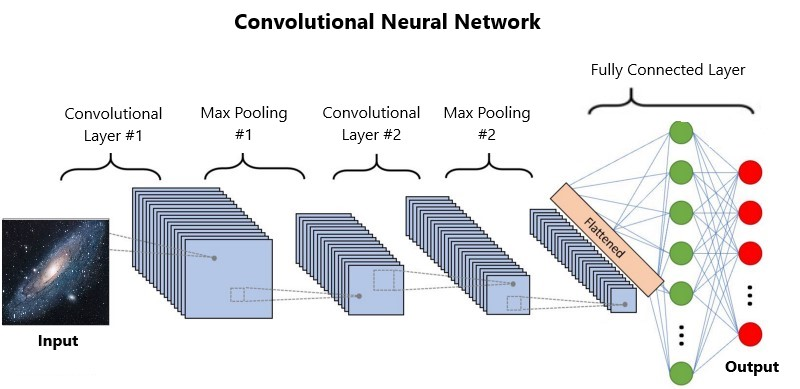
\includegraphics[width=1\textwidth]{../img/cnnModel.jpeg}}
            \label{fig 6: General Schematic of CNN used in image classification} 
            \caption{\label{fig 6:} General Schematic of CNN used in image classification}
        \end{figure}

        \subsubsection{Histological Analysis Limitations}
        Having discussed the potential of artificial intelligence application in different fields, there are a number of challenges that make its use in medicine some what limited and restricted. To be more specific, the challenging work physicians, experts and researchers face when dealing with low-level data is a great issue to consider. Working in such a detail-heavy field can be very challenging as biological systems are well documented to be vigorously complex as Saladin states in his publication \cite{RN21}. Obtaining large amounts of low level data is not a flexible task for this area of study. Whilst manual efforts in this domain are not currently redundant, it may well be in the near future. Such data may have contain too many factors or dimensions to consider as the complexity of the data increases as we move further away from abstract models. Lee et al. \cite{RN20} state that high dimensional data is a problem for researchers to deal with as the ability to analyse may become computationally impossible. Generating tools to decipher data in a much more concise manner for future utilisation is the way which medicine is heading towards at the moment. The analysis of retinal component quantification and the determination of a single layer's degeneration stage all pose the same challenge in this regard and are in dire need of intelligent automation.
        \vspace{3mm}

        Whilst these tasks are clear in terms of objectives, researchers also tend to fall into an abyss of confusion when searching for relevant factors. As difficult as the classification of retinal degeneration may sound, researchers are driven towards investigating elements that are known to have the "biggest" impact on the research. New elements of interests are investigated only if research coincidently stumbles upon them or by trial and error. Additionally, investigating new factors is not as simple in medicine due to the nature of biology. For example, Poplin et al. \cite{RN15} were able to explore if cardiovascular factors can be determined from fundus photographs by applying an algorithm to analyse these images. Obtaining such images is logistically difficult for researchers and not all possible cases can be obtained due to the difficulty of medical imaging. Pattern and trend detection have allowed for new devices to be implemented and have reduced the indecisiveness of experts to invest more resources into a particular study or field. By producing an algorithm for the analysis of retinal H\&E images, we are able to see if the study of cellular structures within the retina is a necessity for investigating the degeneration process.
        \vspace{3mm}

        In addition to the lose of efficiency, the human factor which consists of judgement, decision making and morale is -equally- an important factor to consider. The vast improvements AI has undergone are clear indications that it is a very valuable asset to utilise, but for now it is only assistive and almost acts as a secondary consultant when making impactful decisions in medicine. The fear that a machine is responsible for determining the outcome of a patient's condition is too great for some to grasp, which is understandable at this time. Machines are only machines, with no moral compass to obey by and no sentiments to assist in evaluating a patient's life circumstances. Most decisions in medicine are made to act in the interest of a patient as the field is based on improving an individual's lifestyle. However, those two factors can sometimes collide when deciding on what measure to take in real-life circumstances. An expert or physician gains experience throughout their practical career to make these difficult decisions with a decreased possibility of "collateral damage" for all stakeholder's involved. A machine, or an algorithm to be precise, currently does not have the capability to consider such important factors. A patient, who may suffer form a malignant tumour, opts to pursue treatment for their condition with the full support of the staff involved and their family. When incorporating artificial intelligence into such circumstances, algorithms might not take into consideration the will of patients or the optimism we possess as a species, and so will only be used as an assistive tool in such situations. Vayena et al. \cite{RN22} mention that while artificial intelligence is useful for productivity and potentially eliminating errors, it is important that we stay true to our goals and objectives in its use. When our morals and ethics are compromised for the short-term gain, we will realise that automated algorithms will soon put us at risk and head towards a pessimistic outcome for its future potentials. Generalisation holds potential risks for medicine and the ability to minimise this for automated classification will be largely beneficial for both the algorithm's performance and to the field as a collective.

    \subsection{Problem Statement}
        By summarising the previous discussion on the available literature on retinal degeneration and artificial intelligence, the challenge at hand is clear, retinal degeneration has not been studied extensively using automated classification techniques. There are a number of studies that show the potential of convolutional neural networks in the medical classification field \cite{RN6}\cite{RN13}\cite{RN15}\cite{RN16}\cite{RN14}. The potential of H\&E images is great in paving a pathway to feature discovery of the retina, but is not feasible for manual analysis nor possible to be verified without the use of artificial intelligence. Additionally, available eye protheses for vision-deficient and/or blind patients lack a clear understanding of how the retina degenerates over time. This is a great opportunity to incorporate deep learning into the histological analysis of the retina and provide another insight for all previously mentioned stakeholders.

    \subsection{Aims}
        The lack of "blindness" quantification as well as the need for clear, decisive criteria are major factors that prompt the application of Artificial Intelligence in retinal analysis. We set on an exploration to prove whether or not AI can be implemented on this type of medical images. Initially, this will be conducted on a binary classification task to distinguish blind retina images from those that depict "healthy" or "healthier" ones. We will define the criteria precisely so that identifying the two classes is more of an objective task (rather than subjective as it is currently). The binary classifier shall be tested, evaluated and determine whether such a task is possible.
        \vspace{3mm}
        
        Upon completing this first experimental phase, a more descriptive benchmark will need to be established to identify a multi-classification system for the images. Evaluating the aforementioned binary classifier's performance will be a key step towards determining the optimal multi classifier architecture. Further architecture search studies will be conducted to compare other models to the binary classifier model and will summaries key architectural parameters that affect retinal image classification.  
        \vspace{3mm}
        
        Once an optimal model has been devised, the final stage of experimentation will be an "intra-and-inter observer variability" study. The model will compete against ophthalmology experts (and itself) in evaluating stained retinal images to evaluate its performance on a practical level and further identify potential weaknesses which the model might be facing.
        \vspace{3mm}

        This project will aim to provide key insights into the implementation of CNNs on histologically stained retinal images and into its performance in a "real-world" simulation, ultimately determining its potential clinical application.  

    \subsection{Hypothesis}
        We hypothesise that the convolutional neural network, judging by its previous applications in retinal classification, will be able to classify H\&E images into 2 clearly-distinguishable categories of healthy and non-healthy images of retinae. Additionally, we will be able to build and successfully verify another model capable of classifying images into multiple stages of damage according to a well defined criteria of damage. We may, however, observe discrepancies in the "inter observer variability" tests between the model and the observers as there is no universal criteria for classifying H\&E stained retinal images. We hope to formulate a comprehensive understanding about certain factors that will affect/improve a CNN model's performance on such data (from a computer scientist's perspective), in addition to biological factors that will assist in defining more concise specifications that will expand technology's potential to solve more complex problems.

\pagebreak

\section{Methodology, Research Plans and Preparations}
    \subsection{Development Preparations}
        As discussed previously, many neural networks designed for classification tasks tend to be a variation of Convolutional Neural Networks (CNNs). The development of this particular network is following a carefully devised plan to test out various models capable of producing different classifications.
        \subsubsection{Image Dataset and Pre-Processing}
            The images used for this project are high resolution snippets of feline retinae stained using the Haematoxylin and Eosin (H\&E) method \cite{RN23}. Four initially healthy felines were used as test subjects to obtain their retinae with one eye acting as a control, whilst the other was injected with Adenosine Tri-Phosphate (ATP) to induce artificial blindness. The eyes are implanted with supra-choroidal electrode array (42 electrodes per eye). Once the induced eye was declared functionally blind by conducting a series of tests on the feline's vision ability, the eye is removed, dissected and underwent a series of staining steps. The final product is a collection of retina dissection slides labelled using the following format:
            \begin{center}
                \large{\textbf{W X} L—\textbf{Y\#Z}}
            \end{center}
            where:
            \vspace{3mm}

            \textbf{W}: animal id number 
            
            \vspace{3mm}

            \textbf{X}: left or right eye 
            
            \vspace{3mm}
            
            \textbf{Y}: dissection level number 
            
            \vspace{3mm}
            
            \textbf{Z}: slide number

            \vspace{3mm}

            This information could prove to be valuable upon further investigation of the relationship between the electrode position within the retina and the classification result of that segment. These slides were prepared and provided by the UNSW Graduate School of Biomedical Engineering (GSBME).
            \vspace{3mm}

            As for the imaging process, this was conducted at UNSW Biological Medical Imaging Facility (BMIF) using a high resolution slide scanner. Initially, a selection of 2x168 PNG images was provided by GSBME of these slides (168 per class), however a few issues were encountered in terms of generalising these images for the CNN.
            \vspace{3mm}

            Among the issues that affected the datasets was the irregular positioning of the retina segment. Many images were scanned in a position that allowed the cellular structures to appear parallel to the image's borders. However, other images were not parallel resulting in larger portions of white background and other biological "residue" that would result in unnecessary bias for certain images and affect the classifier's performance if it were to be included in training and/or testing batches. Another justification that led to the retaking of the images was that many of them were taken at different resolutions. Despite this being solved quite well by cropping the images and increasing the zoom on key components, this can also lead to less uniformity between the input samples and, again, un-necessary bias.
            \vspace{3mm}

            Therefore, a new batch of images were scanned using a light microscope to obtain a larger sample of differently-damaged retinae. Training for using the light microscope was provided by UNSW BMIF.
            \vspace{3mm}

            Once the images were ready, the next stage was preparing to label them according to some criteria that defined a \textbf{precise} set of blindness phases. This was conducted with the approval of an ophthalmology expert from the School of Optometry and Vision Science - UNSW. It was important to agree on these definitions with an expert, as we will see later on that this definitive process along with the labelling of the training/validation/testing sets will be a large influencer of the model's performance. The following are the criteria agreed upon for both binary and multi classifiers:
            \vspace{3mm}

            \begin{table}[!h]
                \centering
                    \begin{tabular}{||c c c||} 
                    \hline
                    \textbf{Phase Number} & \textbf{Phase Name} & \textbf{Features} \\
                    \hline\hline
                    0 & Healthy & \begin{tabular}{@{}c@{}}No "biological" abnormalities, strong cellular integrity, \\ no cell migration\end{tabular}\\
                    \hline
                    1 & Blind & \begin{tabular}{@{}c@{}}"Biological" abnormalities, weak cellular integrity,\\ cell migration\end{tabular}\\
                    \hline
                    \end{tabular}
                \caption{\label{fig:4} Binary Classification Criteria (RetinaNET v0.1)}
            \end{table}

            \begin{table}[!h]
                \centering
                    \begin{tabular}{||c c c||} 
                    \hline
                    \textbf{Phase Number} & \textbf{Phase Name} & \textbf{Features} \\
                    \hline\hline
                    0 & Healthy & \begin{tabular}{@{}c@{}}No "biological" abnormalities, strong cellular integrity,\\no cell migration\end{tabular}\\
                    \hline
                    1 & Mildly Damaged & \begin{tabular}{@{}c@{}}Some "Biological" abnormalities, mildly-disorganised layers, \\ some cell migration\end{tabular} \\
                    \hline
                    2 & Blind & \begin{tabular}{@{}c@{}}Many "Biological" abnormalities, weak cellular integrity, \\  cell migration\end{tabular}\\
                    \hline
                    \end{tabular}
                \caption{\label{fig:4} Multi Classification Criteria (RetinaNET v1.0)}
            \end{table}
            
            The binary classifier rules are objective and can clearly distinguish between the two phases that are defined. The expectations for this model are high and should be able to perform very well. As for the multi classifier, its criteria may face challenges in distinguishing these phases and are subject to future improvements. The healthy phase is defined identically to the binary classifier's healthy phase. The confusion arises when splitting the binary's blind phase into 2 distinct phases. The distinction between a mildly damaged versus a completely blind retina is a subjective matter. The challenging issue is the "fluidity" between the two phases (1,2) and no "outstanding" border that can universally define these phases.
            \vspace{3mm}
            
            Finally, the images were labelled according to the rules previously discussed. Due to the project's limitations and the large number of images that need to be labelled, this was conducted by a retinal 'novice' (the author). All of the training and validation images were labelled by the novice. However, a testing set was not only labelled by the novice, but also by 2 retinal experts, one who was complicit in the drafting of the blindness criteria and another who had no prior knowledge of the project. This framework would allow for extensive statistical analysis of the model's and experts' performances as well as approximating how well a model would perform in a real life situation.
            \vspace{3mm}       

            The following is an overview of the new dataset (both binary and multi) produced with the light microscope:
            \begin{table}[h]
                \centering
                    \begin{tabular}{||l l|l l|l l|l l||}
                    \hline
                        \multicolumn{2}{c}{\textbf{Training}} &
                        \multicolumn{2}{c}{\textbf{Validation}} &
                        \multicolumn{2}{c}{\textbf{Testing}} &
                        \multicolumn{2}{c}{\textbf{Total}}\\
                        {\textit{Binary}} & {\textit{Multi}} & \textit{{Binary}} & \textit{{Multi}} & \textit{{Binary}} & \textit{{Multi}} & \textit{{Binary}} & \textit{{Multi} } \\
                        \hline\hline
                        222 & 463 & 95 & 134 & 83 & 83 & \textbf{400} & \textbf{680} \\
                    \hline
                    \end{tabular}
                    \caption{\label{fig:4} Dataset sizes for both classifiers (\# of images)}
            \end{table}

            \nopagebreak

                \begin{table}[h]
                    \centering
                        \begin{tabular}{||l l|l l l||}
                        \hline
                            \multicolumn{2}{c}{\textbf{Binary}} &
                            \multicolumn{3}{c}{\textbf{Multi}} \\
                            {\textit{Healthy (0)}} & {\textit{Blind (1)}} & \textit{{Healthy (0)}} & \textit{{Mildly Damaged (1)}} & \textit{{Blind (2)}} \\
                            \hline\hline
                            168 & 149 & 186 & 255 & 156 \\
                        \hline
                        \end{tabular}
                        \caption{\label{fig:4} Distribution of data-points for both classifiers (\# of images)}
                \end{table}


            \nopagebreak
            As previously discussed, obtaining large amounts of data for an AI model is extremely important in order to achieve interesting results. In this case, the distribution of the data was relatively even for the binary classifier which would allow for an unbiased learning process. However, the multi classifier had a fair margin between the three classes' distribution, prompting for some additional pre-processing to even this distribution out. Data augmentation of the multi-dataset allowed for an increase in the number of images for phases 0 and 2. Such techniques include increasing the lighting condition of the images that appear to be dark. This was an issue that arose when using a light microscope as an imaging tool, hence this augmentation produces more images with higher lighting and improve the learning process.
            \vspace{3mm}

        \subsubsection{Software Configurations and Setup}
            The development of this neural network will depend on a powerful Deep Learning framework called TensorFlow along side Python 3.6.3. The options it offers for convolutional neural networks are vast and provides a flexible set of programming features that easy the calculus-dependent computations. The choice of Python was straight forward as the language is universally supported for many different programming applications and has a good reputation for AI projects.
            \vspace{3mm}

            Primarily, the development and training/testing process will be conducted on a personal device for fast and easy access, however there are hardware issues to consider for such a project. Deep learning projects are notoriously known to be computationally-expensive and time consuming when it comes to training and testing models. The personal device specifications are not suited for such tasks and high-performance computers may need to be used in the future (e.g. UNSW Katana Clusters).      

        \subsubsection{Model Performance Evaluation and Statistical Analysis}
            As is illustrate in Table 5 above, the training and validation split is 70-30. This split is subject to further modifications for future models. Literature suggests that this is usually the optimal ratio when it comes to splitting the data. Initially, evaluating a model's performance will depend on interpreting the training and validation accuracy and loss. These were collected using TensorBoard (TensorFlow's statistical dashboard). This will give an early indication if a model is appropriate for the set classification task and will move to the next stage of evaluation. A 83-image testing set that has not been seen before by the model (neither training nor validation). 
            \vspace{3mm}
            
            A number of statistical scores will be taken on the model's performance on the testing set, such as accuracy, loss and average weighted F1 scores. Accuracy is defined as the ratio of \textbf{TRUE} predictions an observer has made to the total number of predictions. Loss can be defined as the level of confidence a classifier has reached when predicting a specific data-point. As will be discussed later on, the SoftMax function which outputs a probability for each class ranges between 0 and 1. The class with the higher probability is concluded to be the class of the input image. However, a probability score of 0.99 as opposed to 0.89 suggests that the model is more confident in the first case. Thus, it is important to give the model an indication of whether it is traveling in the correct direction or not, hence lowering the loss score. These two metrics are the standard when evaluating a deep learning model. 
            \vspace{3mm}
            
            The weighted F1 score is defined as:
            \begin{center}
                \textbf{Weighted-F1 = {\huge $ \frac{\Sigma_{i \in C}  (\vert{i}\vert . F1_{i})}{\Sigma_{i \in C}  (\vert{i}\vert)}$}}\\
            \end{center}
            where :
            \vspace{3mm}
            
            \textbf{C}: the set containing all classes/phases defined for the classifier (e.g. phases 0-1 for binary, 0-1-2 for multi)
            
            \vspace{3mm}
            
            \textbf{F1} = { $\frac{2 . Precision . Recall}{Precision + Recall}$}
            
            \vspace{3mm}
            
            \textbf{Precision} = { $ \frac{tp}{tp + fp}$}\footnote{Refer to Abbreviations section for full clarification}
            
            \vspace{3mm}
            
            \textbf{Recall} = { $ \frac{tp}{tp + fn}$}
            
            \vspace{3mm}

        A f1 score is an excellent measure to get an idea of how the model is performing with respective to both sensitivity and specificity (recall and precision). However, a pure F1 score will not be meaningful in our multi classification, as the distribution of the data-points is some what skewed (apparent in table 6). Adjusting to this distribution by applying a weighting to each class will help determine the model's performance in identifying relevant classes that appear in the dataset. 
            
    \newpage
    \subsection{Proposed Solution}
        \subsubsection{Binary Classifier Architecture (RetinaNET v0.1)}
            This initial design is the precursor to the optimal design of having a network that can quantify the level of retinal damage a low-level cellular image of a retina shows. The design of this preliminary model can be divided into the following:
            \begin{itemize}
                \item 3 Convolutional blocks: each block is made up of the following:
                    \begin{itemize}
                        \item 1 Convolutional layer (per block): These layers are the first interaction the images have with the first two block layers having a kernel size of 3x3 pixels and number of outputs tallying at 32. The third block layer comprises another 3x3 kernel, however has a larger number of filters, 64. 
                        \item 1 Pooling layer (per block): these layers are the immediate suffix components to the convolutional layers acting as the optimising component that will reduce the computational load on the model and hence decrease any overfitting the model might endure. 
                        \item 1 ReLU Activation function: a simple yet effective function to map the output of the convolutions and create complex relationships that have been learned from the data. This function is typically the first choice as an activation function for such tasks.
                    \end{itemize}
                \item 1 Flattening layer: for development framework (TensorFlow) purposes of dimensionality conformity when transitioning from the convolutional sections to the fully-connected layer.
                \item 2 Fully connected layers: these act as the artificial network of neurons that will eventually output whether the input image to the CNN is classified as blind or normal.
                \item SoftMax Activation function: to scale the 2 outputs which the last fully-connected neuron layer (or logits layer) produces to a probability score between [0, 1]. This is done according to the following function definition:
                \begin{center}
                    \textbf{SoftMax(i) = {\huge $ \frac{e^{i}}{\Sigma_{j} e^{j}}$}}\\
                \end{center}
            \end{itemize}
            The weighting parameters are initially selected to be random and upon further training iterations, they begin to adapt in order to distinguish between the two classes. This model is based on previous applications of CNNs in retinal classification tasks and will be prone to future modifications when the research phase for RetinaNET v1.0 begins.
            \vspace{3mm}

            The appendix contains a full summary of the model's hyper-parameters

        \subsubsection{Multi Classifier Architecture (RetinaNET v1.0)}
            An architecture search study was conducted for the multi classifier. Due to ambiguous distinctions between some of the classes (e.g. classes 1-2), it is essential that the model architecture is able to capture the key features necessary for determining these boundaries. A more complex model than the binary classifier is needed and a study of key architectural components was conducted. The following is a summary of the architecture search completed to obtain the optimal design for the multi classifier:
            \vspace{3mm}
            \pagebreak

            \begin{figure}[h!]
                \centerline{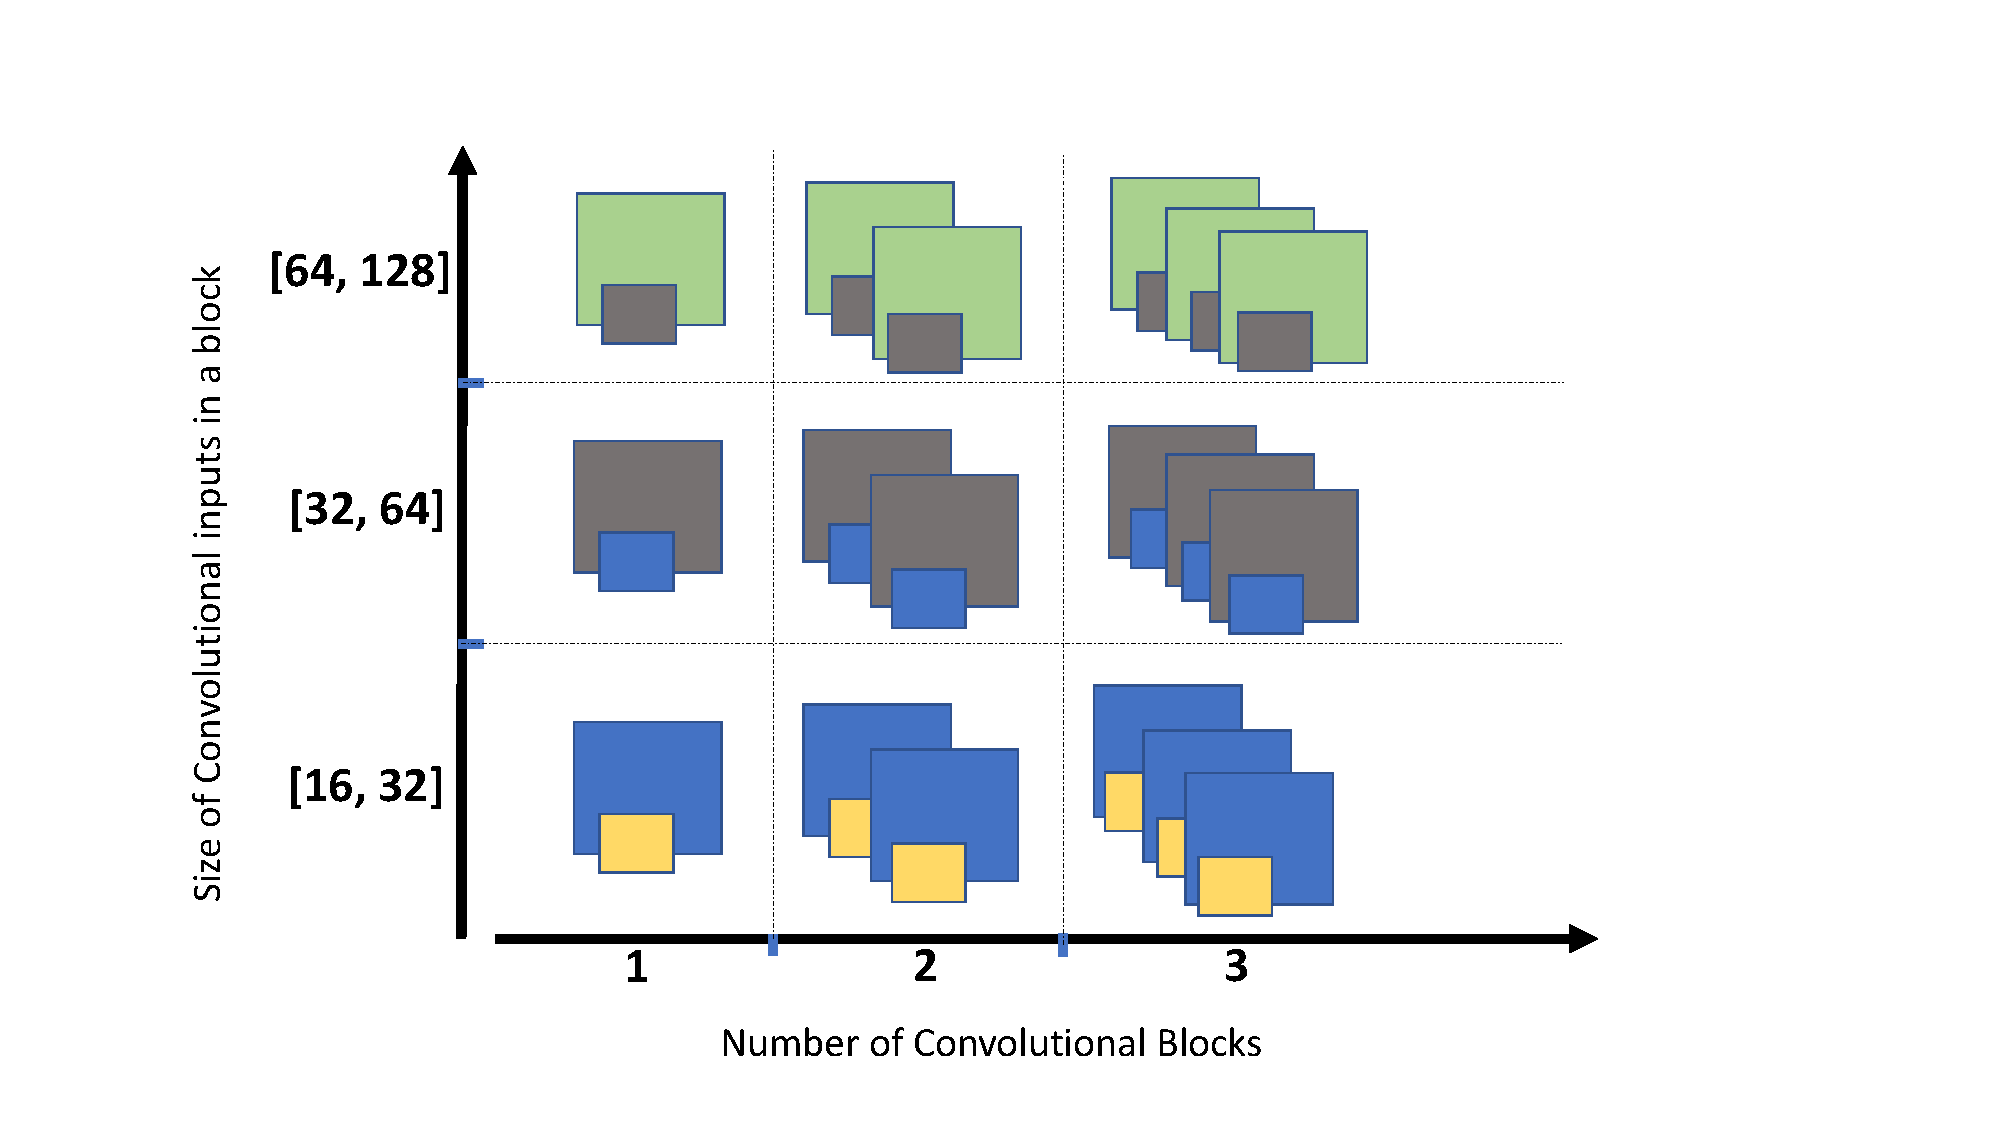
\includegraphics[width=1\textwidth]{../img/map.pdf}}
                \label{figX: Architecture Search Plan} 
                \caption{Architecture Search Plan}
            \end{figure}

            This experiment is necessary due to the "black-box" nature of a CNN. Literature has not been able to provide evidence backing claims that certain parameters affect the performance of a neural network. The manner in which an optimal architecture is achieved for CNNs is through trail-and-error \cite{RN13}. It is understood that increasing the complexity of a model will assist in learning new features until overfitting occurs. Whereas, if a network is too simple, it will not learn enough features to be effective enough. Thus, it is a "balancing estimation" of the parameters that affect these factors that will essentially define a model\'s performance (from an architectural aspect that is). The 2 parameters chosen for this study are:

            \begin{itemize}
                \item Number of Convolutional blocks.
                \item The output size of the 2 convolutional layers in each block. \footnote{A constant assumption made (in this study) is that the number of convolutional layers in a single block is \textbf{2}}
            \end{itemize}
            \vspace{3mm}

            The first parameter controls the "depth" of our convolutional segment of the network, increasing these parameters will result in additional convolutional layers. Once again, increasing this will help the model learn complex relationships until overfitting beings to occur. The second parameter affects the size of the tensors (vectors) that are passed into the convolutional layers, which will either increase the field of view that is convoluted in each layer. Conventionally, this parameter increases throughout the network. However, due to computational constraints placed on this project, it was necessary to use the same inputs for all blocks included in each case for the architecture study. For example:
            \vspace{3mm}
            
            \textbf{IF} (number of convolutional layers = 2 {AND} size of convolutional inputs = (64,128)) 

            \vspace{3mm} 

            \textbf{THEN}:

            \begin{center}
                $(Conv_{11}(64) \rightarrow Conv_{12}(128)) \Rightarrow (Conv_{21}(64) \rightarrow Conv_{22}(128))$.
            \end{center}

            As for the remaining components of the CNN (hyperparameters, other architectural factors), these are identical to the binary classifier with the exception of the Logits layer containing 3 values (as opposed to 2) that are normalised by a SoftMax function. These represent the 3 classes the multi classifier aims to classify the images.  

        \newpage
        \subsubsection{Development Plan}
        The development cycle for this project will follow an agile strategy that will help maintain, improve and evaluate the proposed solution to this problem. The following is an outline of the process:
    
        \begin{itemize}
            \item The imaging/re-imaging of the retinal segments slides. 
            \item Code development: this is an iterative process and will follow an agile strategy where the code is reviewed weekly individually to investigate issues and problems obstructing development. This will also include the review of the model and its code, its performance and methods of optimisation and improvements.
            \item Running local testing rounds: this is to evaluate the performance of the model and collect statistical data that helps identify its performance and evaluates optimisation methods.
            \item Meeting up with supervisors and experts: a fortnightly, scheduled meeting to discuss the current status and progress of the model, development performances, testing results. This will also include discussing previous iterations of testing of the current model as well as previous models and current statistical scores. 
            \item The repetition of previous 4 steps fortnightly, following an agile style of continuous development and improvement.
        \end{itemize}

        This setup gave the models the maximum potential to be improved and fine-tuned, and ultimately, achieving an optimal design that can be implemented for future projects. The development phase of the code will be documented on GitHub.
        \vspace{6mm}
       

    \subsubsection{Risk Assessment}
        Since this model is evaluating real-life data of retina images, the risk lies in the accuracy and precision of the classifications. Future applications of this model could be clinical and in future researches that while rely on the findings of the network. A miss-classification of images could pose risks for these applications and undermine their findings. Additionally, clinicians may apply this tool in their practices for patient evaluation and the results will affect the outcome of appointments and operations. It is important that the performance of the model is verified and validated, using feature extraction effectively and not determining results by chance.

\pagebreak

\section{Results}
\subsection{Binary Classifier}
    The preliminary results of RetinaNET v0.1 were promising, as the model was able to reach an average of 100\% training accuracy, 87.6\% validation accuracy while achieving an average minimum validation loss of 25\% \footnote{\textbf{NOTE:} Training and Validation Datasets were labelled by Novice, Testing by an expert}. These results were run 10 times, with each training round consisting of 600 iterations. This number was later reduced to 400, as the validation loss began to increase at this particular range (suggesting 400 iterations as the overfitting "point-of-no-return"). Table 7 demonstrates the results of RetinaNet0.1:

    \begin{table}[!h]
        \centering
            \begin{tabular}{||c c c||} 
            \hline
            \textbf{Training Accuracy (\%)} & \textbf{Validation Accuracy (\%)} & \textbf{Validation Loss (\%)} \\
            \hline\hline
            1.000 & 0.876  & 0.25 \\
            \hline
            \end{tabular}
        \caption{\label{fig:4} Average Training Accuracy, Validation Accuracy and Loss values for RetinaNET v0.1}
    \end{table}

    Training and validation curves were obtained from TensorBoard and are shown below:
    \begin{figure}[h!]
        \centerline{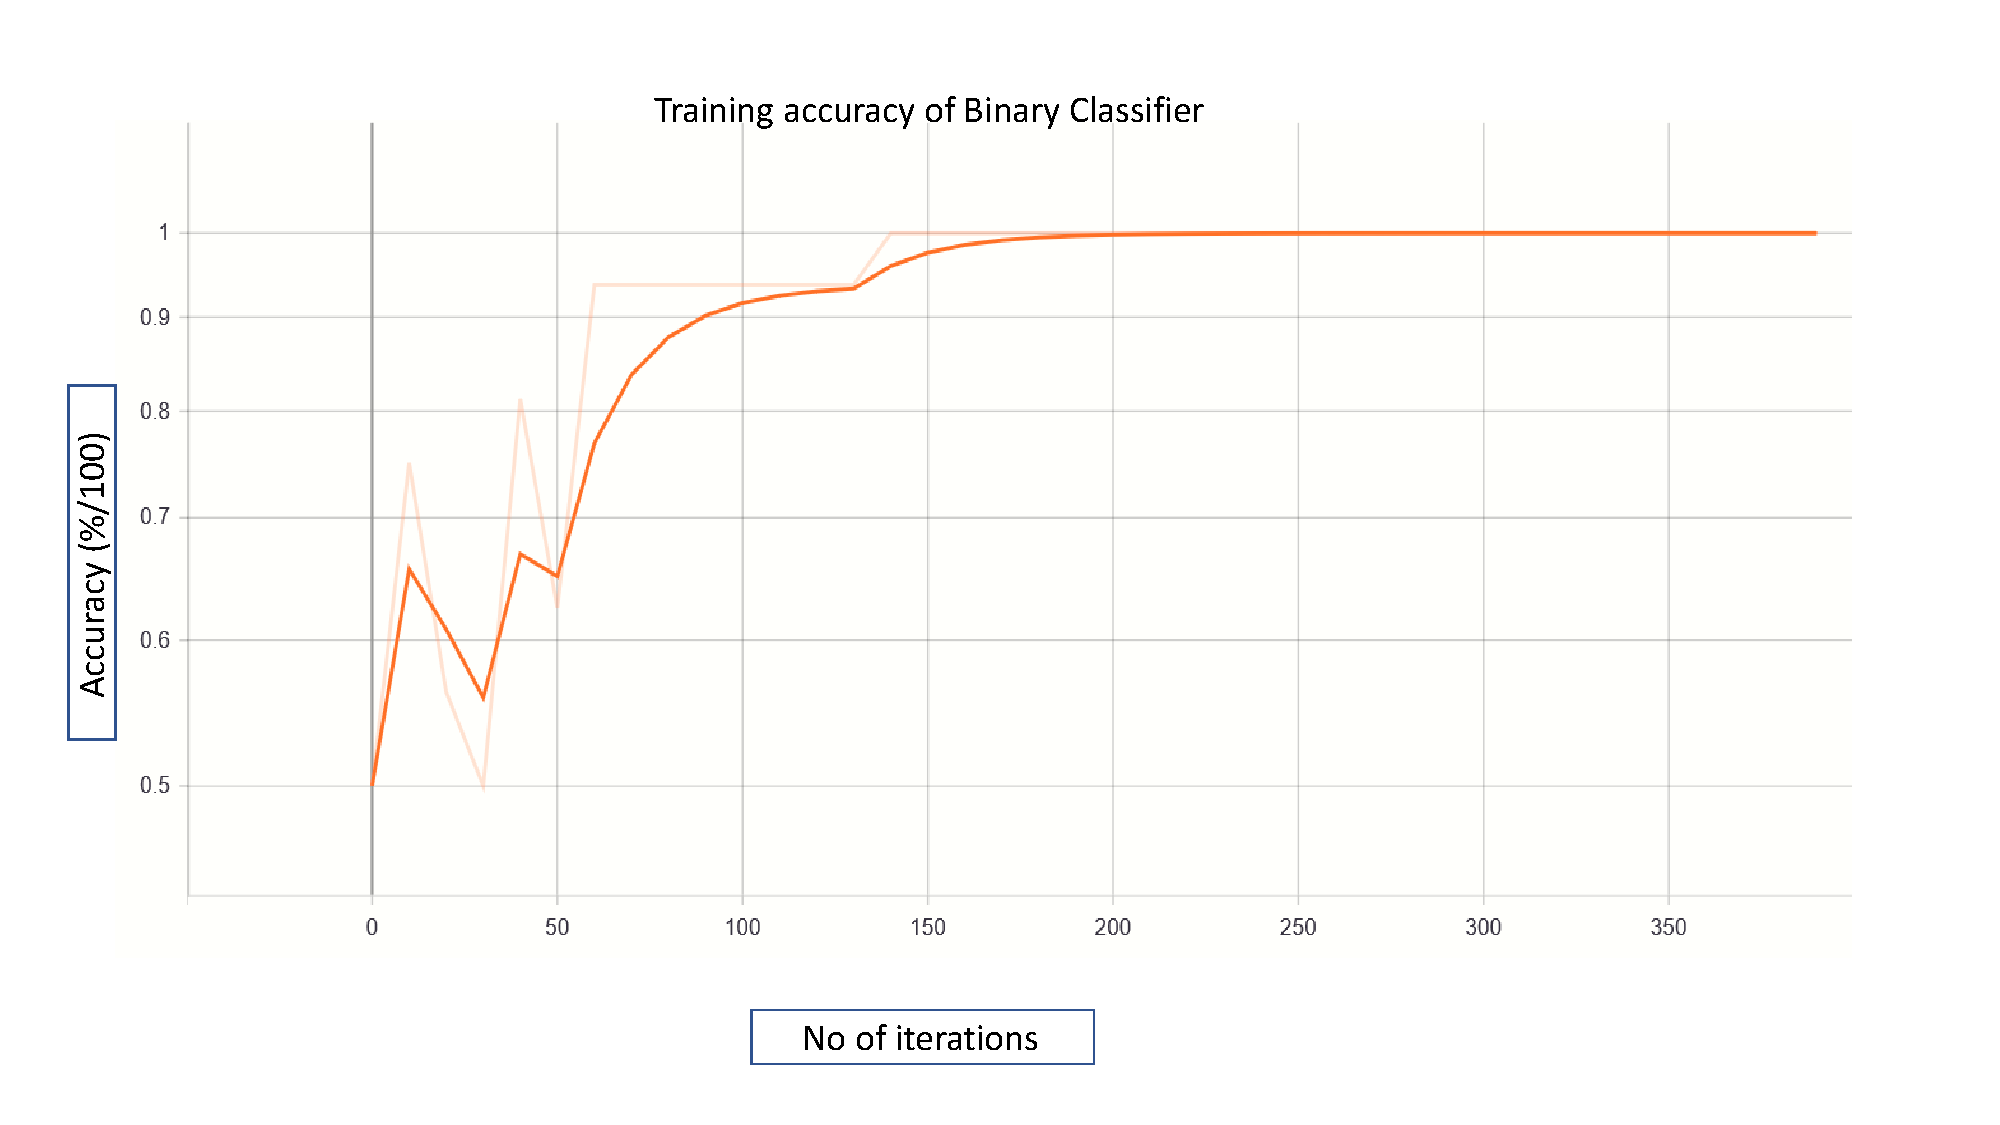
\includegraphics[width=0.8\textwidth]{../img/results/binTraining.pdf}}
        \label{figX: Binary Training Accuracy Curve} 
        \caption{Binary Classifier Training Accuracy Curve}
    \end{figure}
    \begin{figure}[h!]
        \centerline{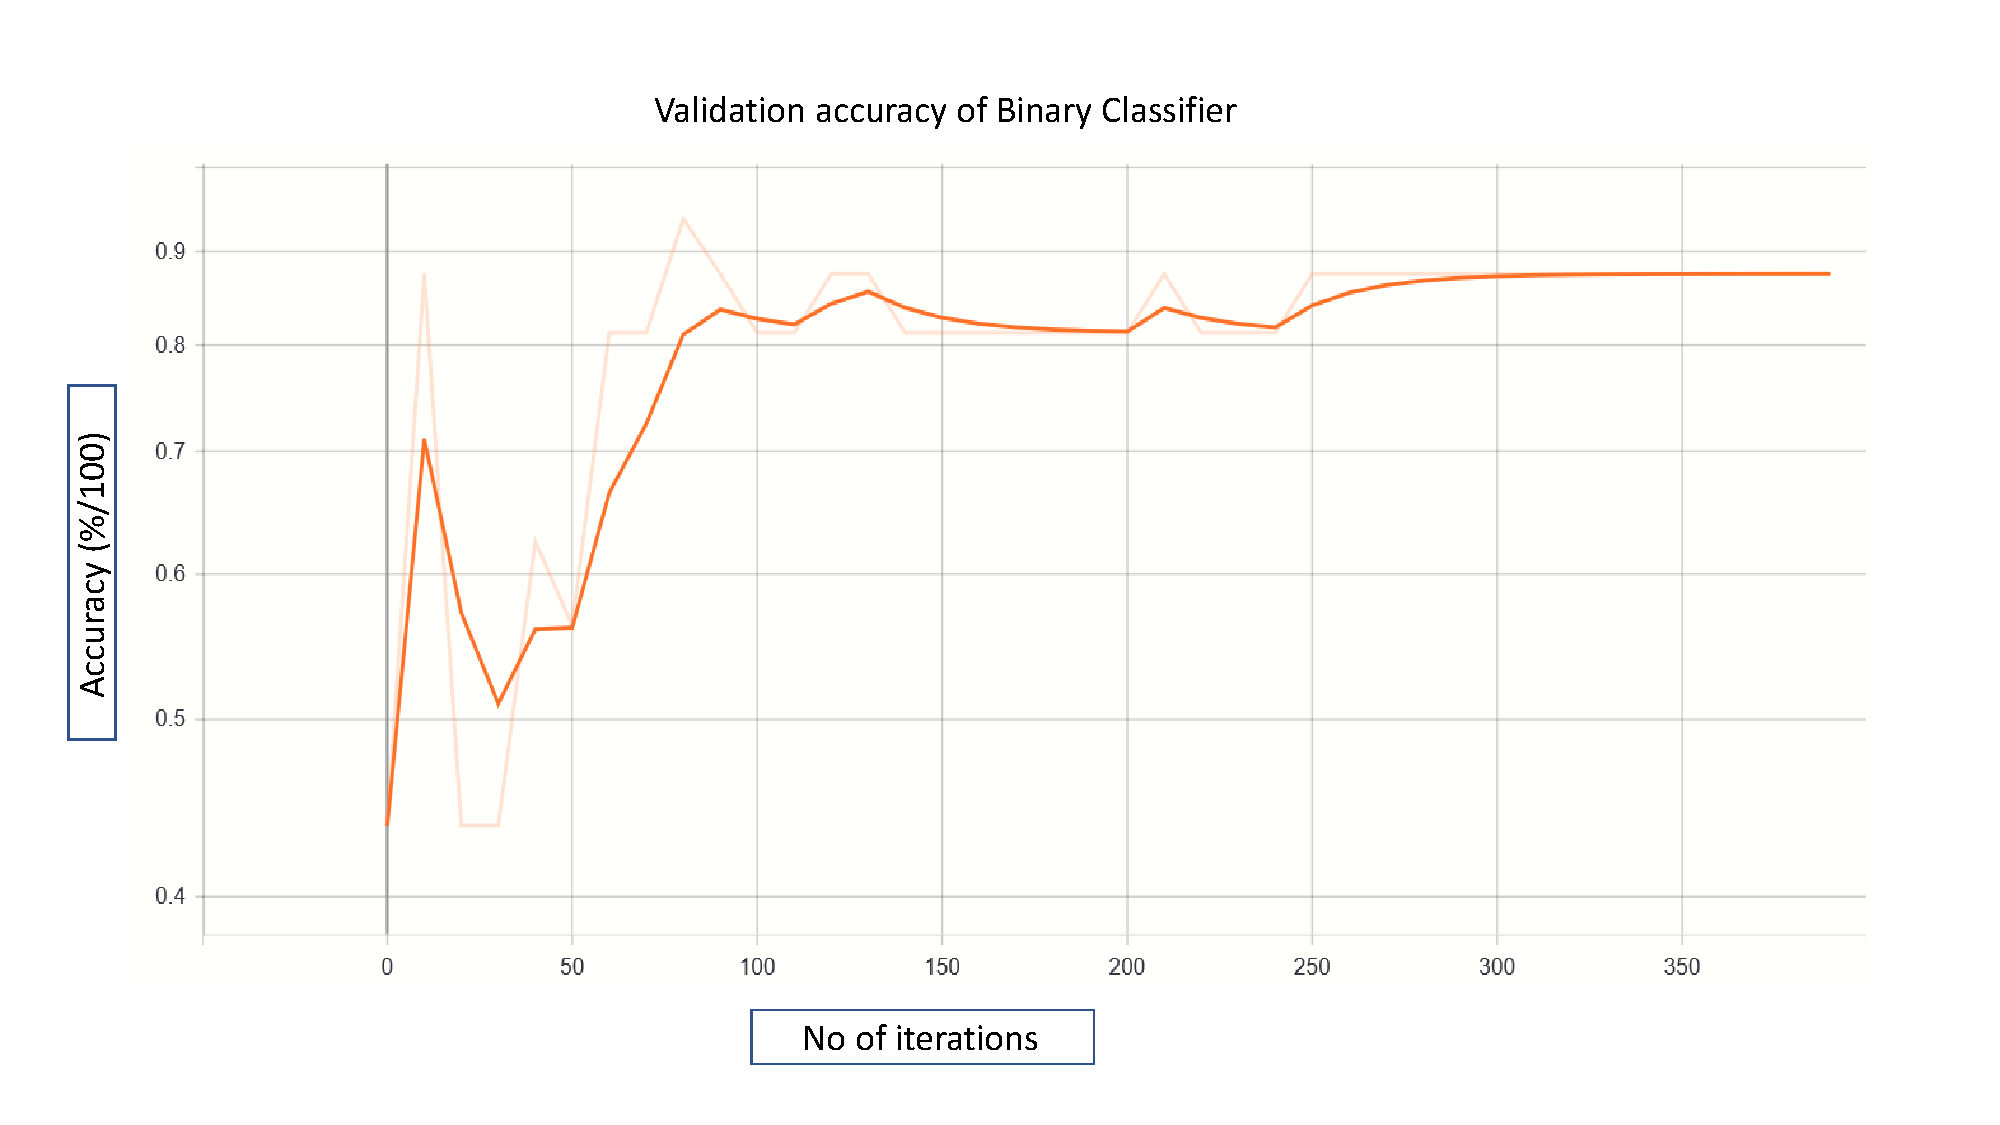
\includegraphics[width=0.8\textwidth]{../img/results/binValidationAcc.pdf}}
        \label{figX: Binary Classifier Validation Accuracy Curve} 
        \caption{Binary Classifier Validation Accuracy Curve}
    \end{figure}
    \begin{figure}[h!]
        \centerline{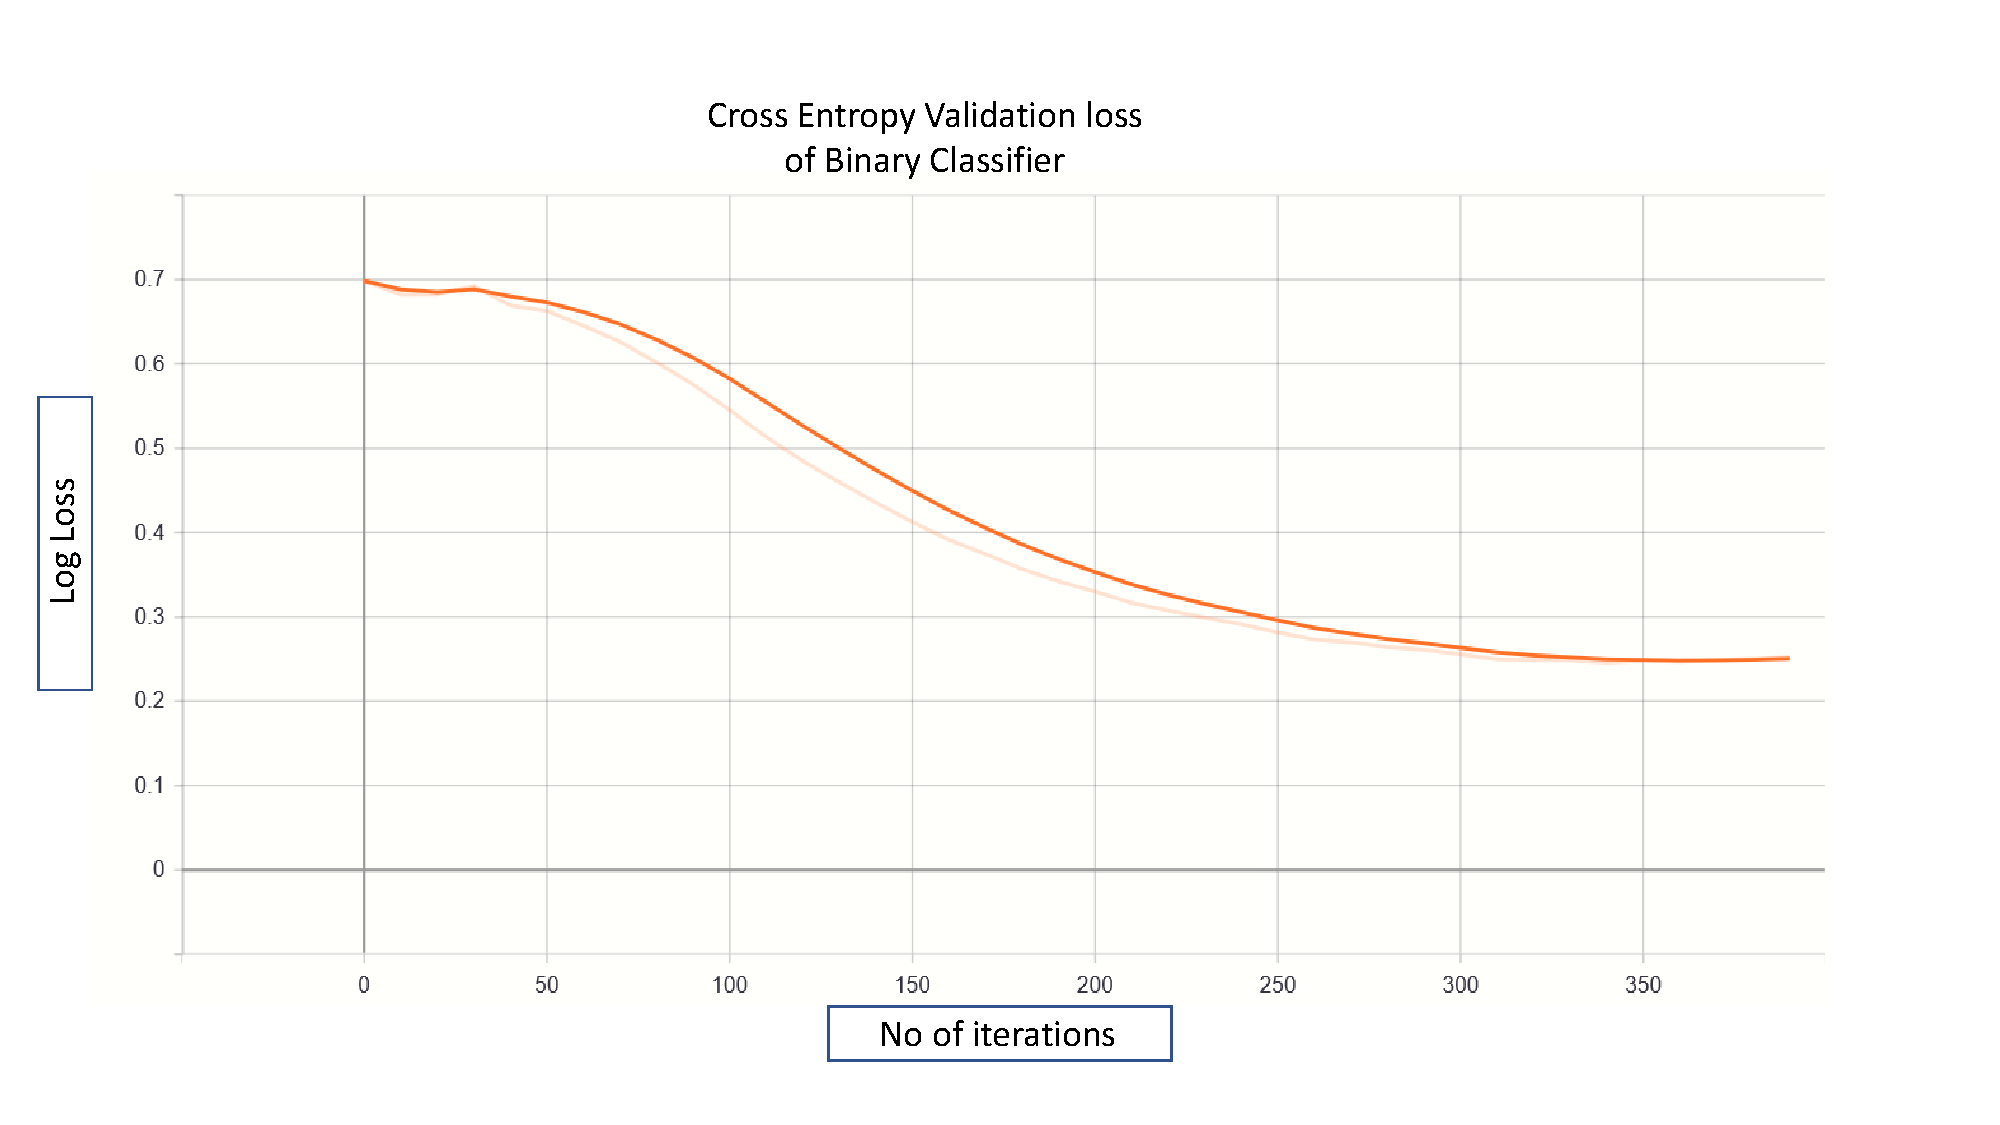
\includegraphics[width=0.8\textwidth]{../img/results/binValidationLoss.pdf}}
        \label{figX: Binary Classifier Validation Loss Curve} 
        \caption{Binary Classifier Validation Loss Curve}
    \end{figure}

    An Exponential Moving Average (EMA) known in TensorBoard as a "Smoothing function" with a scale of 1 produces the darker curve observed in tables 5-7. The lighter curve in the same tables are the raw values. This EMA was applied to identify the trend of the curves as raw values usually result in peaks and troughs that disturb the continuity of the curves.
    \vspace{3mm}  

    As for the testing evaluation phase, out of the 83 images used, the model was able to correctly distinguish 93\% for normal images and 82\% for the blind. Initially, the image dataset had a common theme with some of the images containing un-necessary residue that would affect the behaviour of the model. Upon the elimination of these artefacts (via cropping and other data pre-processing techniques), the testing accuracy rose immediately and indicated that a model for binary classification is in-fact accurate and precise.\vspace{3mm}

    \begin{table}[!h]
        \centering
            \begin{tabular}{||c c||} 
            \hline
            \textbf{Testing Accuracy for Normal Images (\%)} & \textbf{Testing Accuracy for Blind Images (\%)} \\
            \hline\hline
            0.930 & 0.820 \\
            \hline
            \end{tabular}
        \caption{\label{fig:4} Average Testing Accuracy for Normal and Blind Images of retinae for RetinaNET v0.1}
    \end{table}
    \subsection{Multi Classifier}
        \subsubsection{Architecture Search}
        Figure 8 is a summary of the results obtained when conducting the Architecture Search experiments on the Multi-classifier. The most efficient method to test all 9 architectures accurately and to get an idea of the performance of each was to train all models and then run them on the unseen testing set, measuring weighted F1 scores as well as obtaining the confusion matrix on this same set. Fortunately, the search process was able to distinguish a clearly dominant model that was able to achieve a high weighted-F1 score as well as a well balanced confusion score. This model has the 2 convolutional blocks with input sizes of 64 and 128 for each convolution respectively in each block.  

        \newpage
        \begin{figure}[h!]
            \centerline{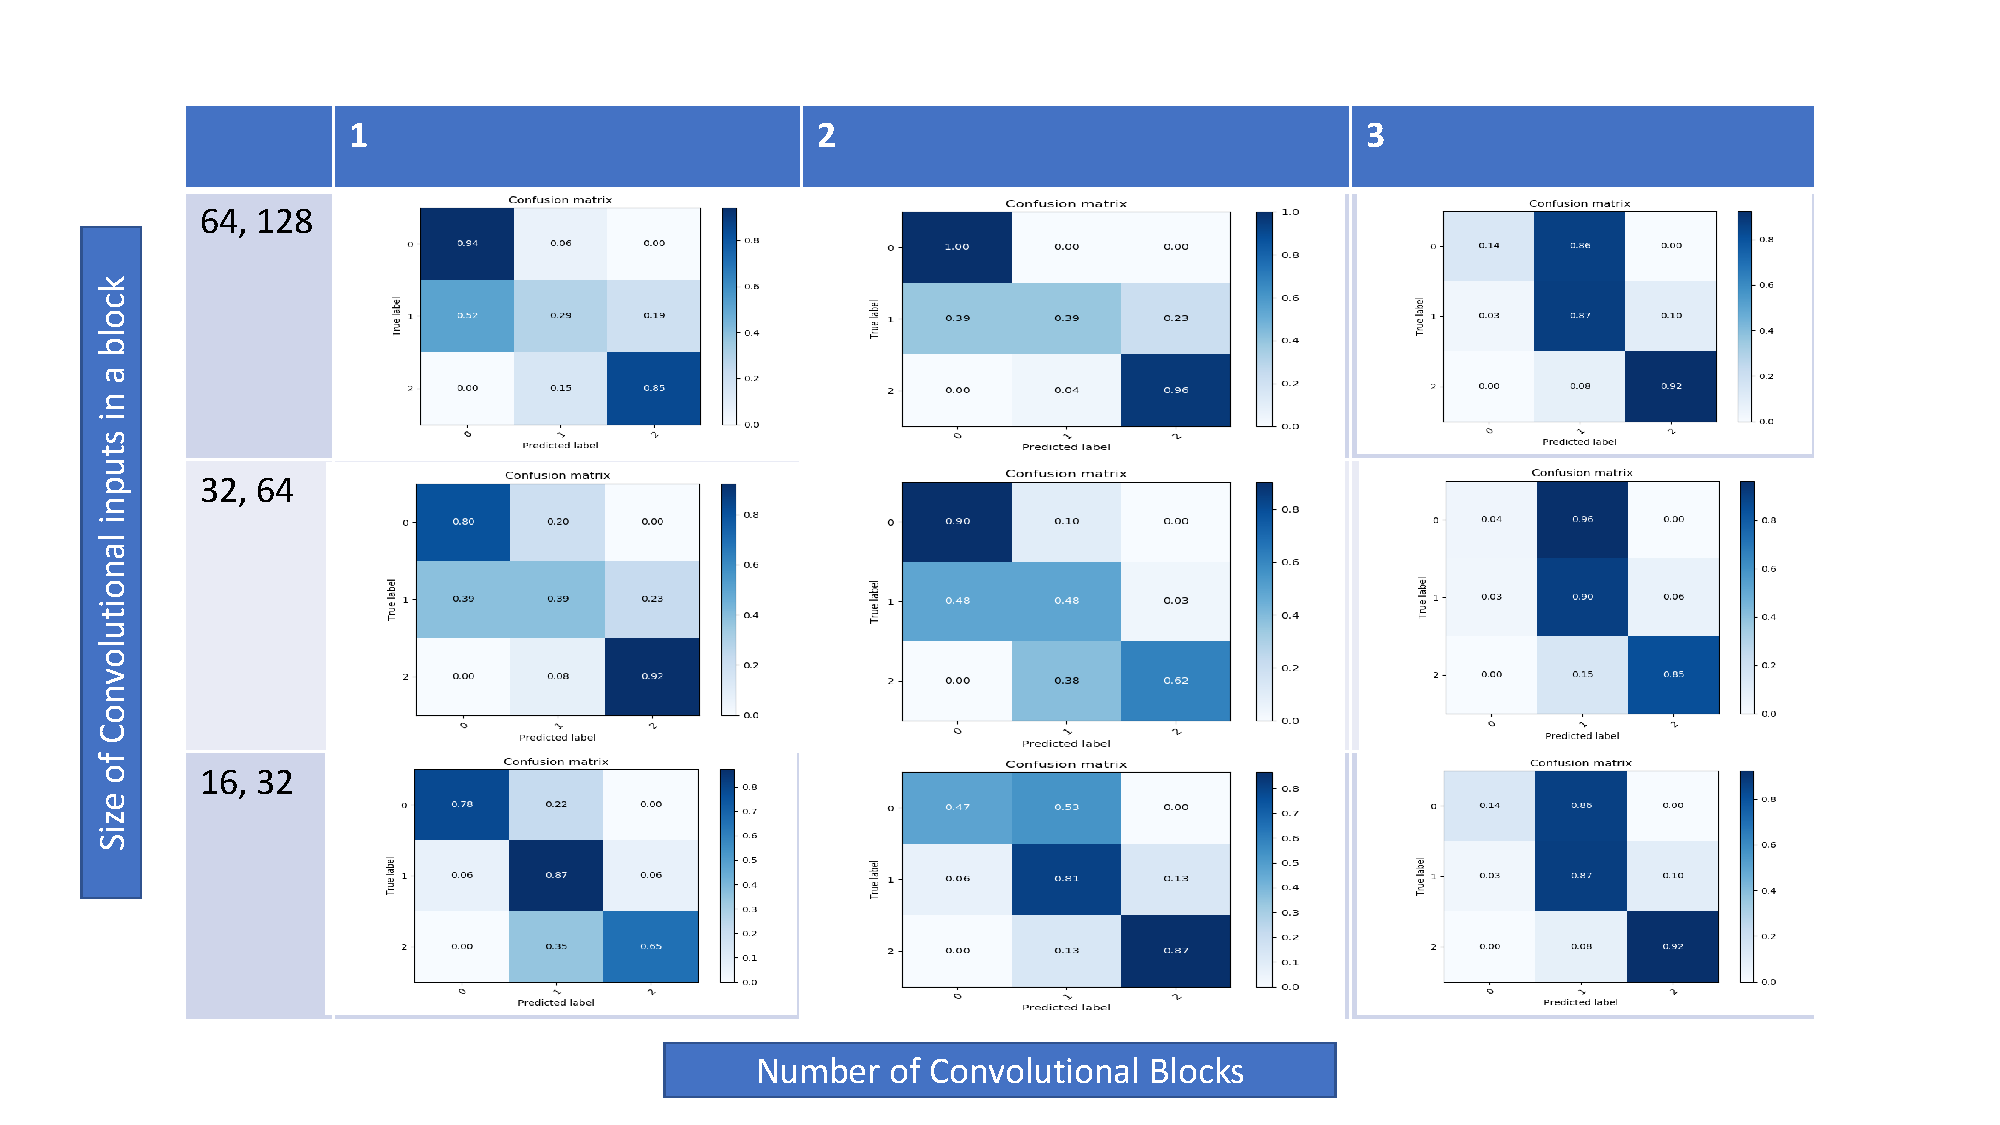
\includegraphics[width=1\textwidth]{../img/results/archi.pdf}}
            \label{figX: Architecture Search Results} 
            \caption{Architecture Search Results}
        \end{figure}

        \begin{table}[!h]
            \centering
                \begin{tabular}{||c || c c c||} 
                \hline
                 & \textbf{1} & \textbf{2} & \textbf{3} \\
                \hline\hline
                \textbf{64, 128} & 0.734 & 0.820  & 0.570 \\
                \textbf{32, 64}  & 0.746 & 0.703  & 0.488 \\
                \textbf{16, 32}  & 0.771 & 0.712  & 0.570 \\
                \hline
                \end{tabular}
            \caption{\label{fig:4} Weighted F1 Scores for the different RetinaNET v1.0 architectures}
        \end{table}

        The following curves are the training and validation accuracies and loss for the optimal multi classifier obtained from the architecture search:
        \begin{figure}[h!]
            \centerline{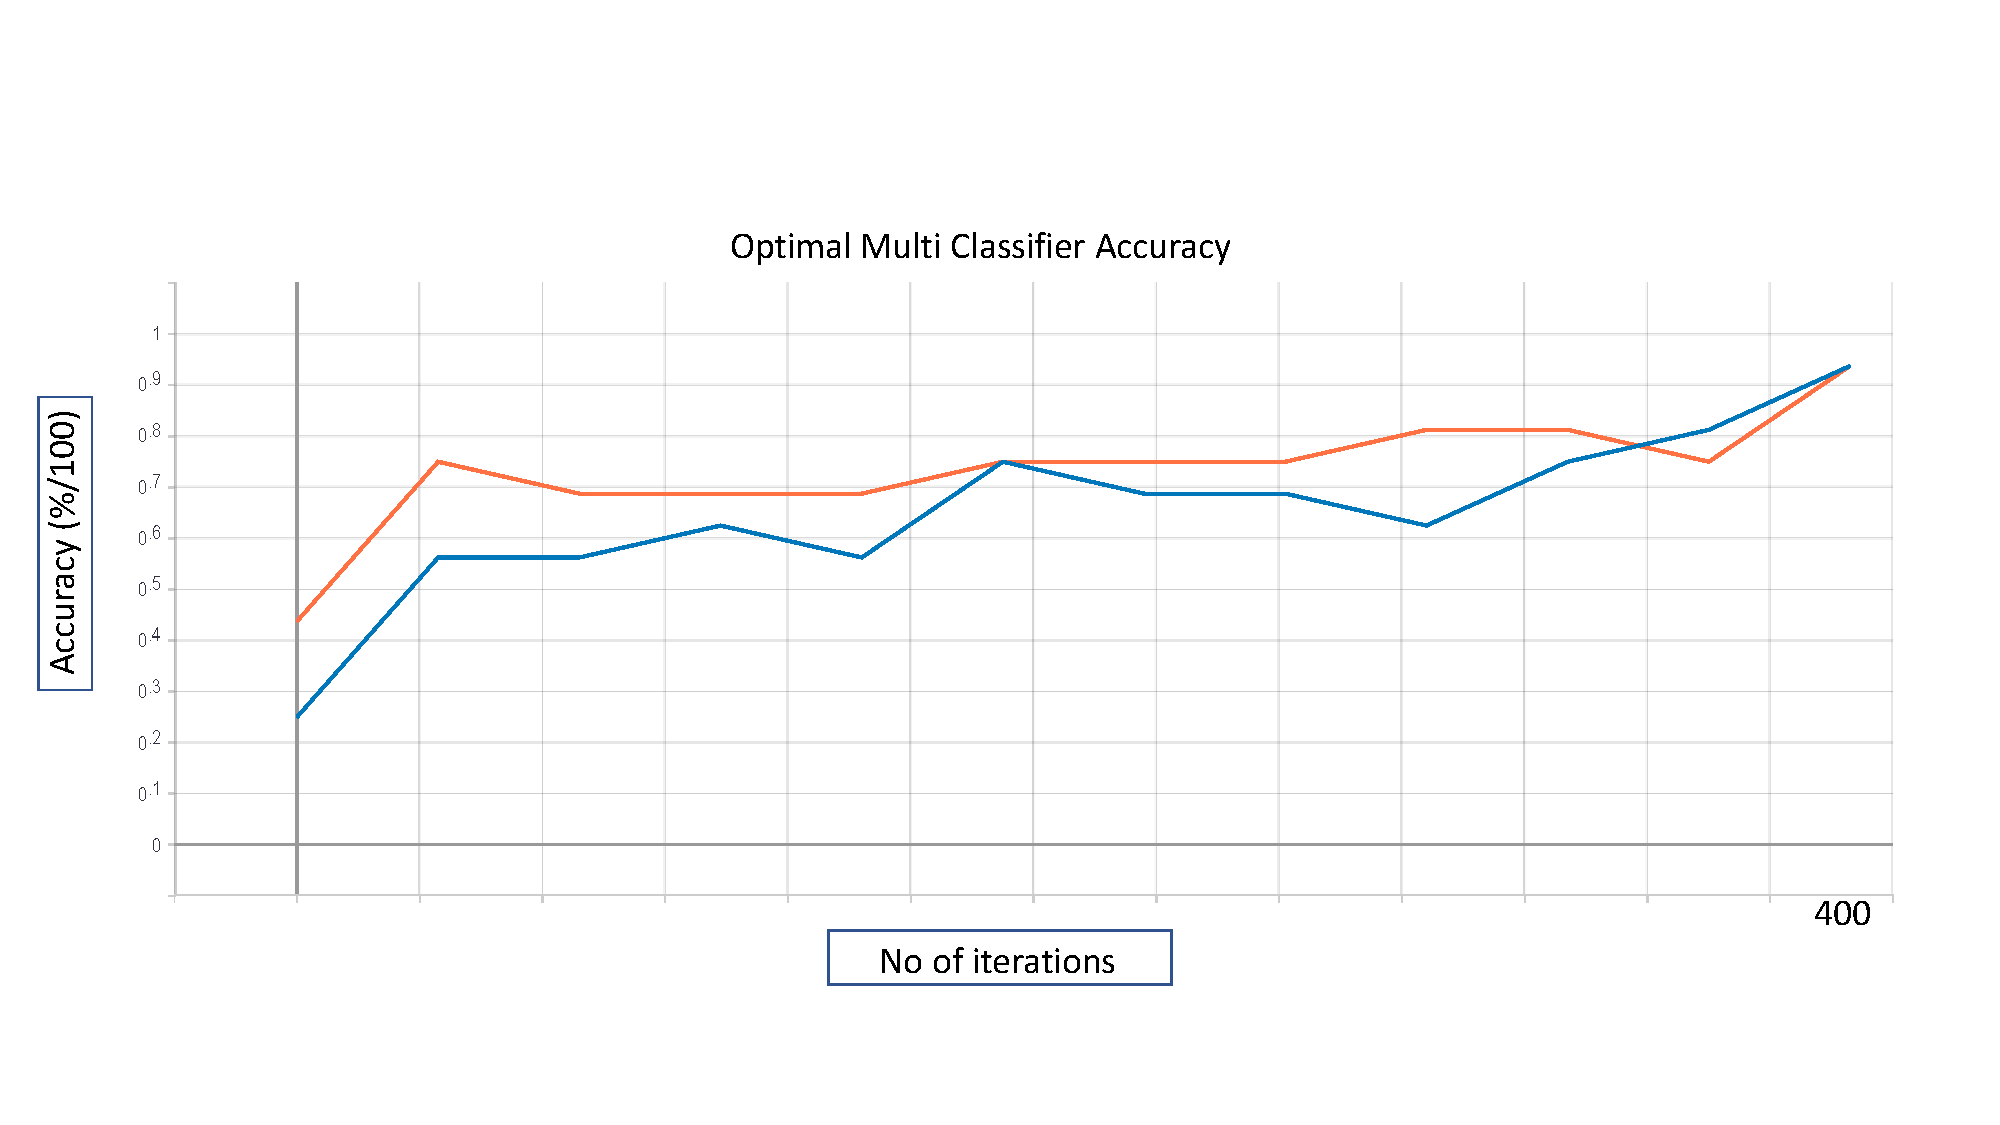
\includegraphics[width=1\textwidth]{../img/results/multiAcc.pdf}}
            \label{figX: Optimal Multi Accuracy Curves} 
            \caption{Optimal Multi Accuracy Curves; blue:training, orange:validation}
        \end{figure}
        \begin{figure}[h!]
            \centerline{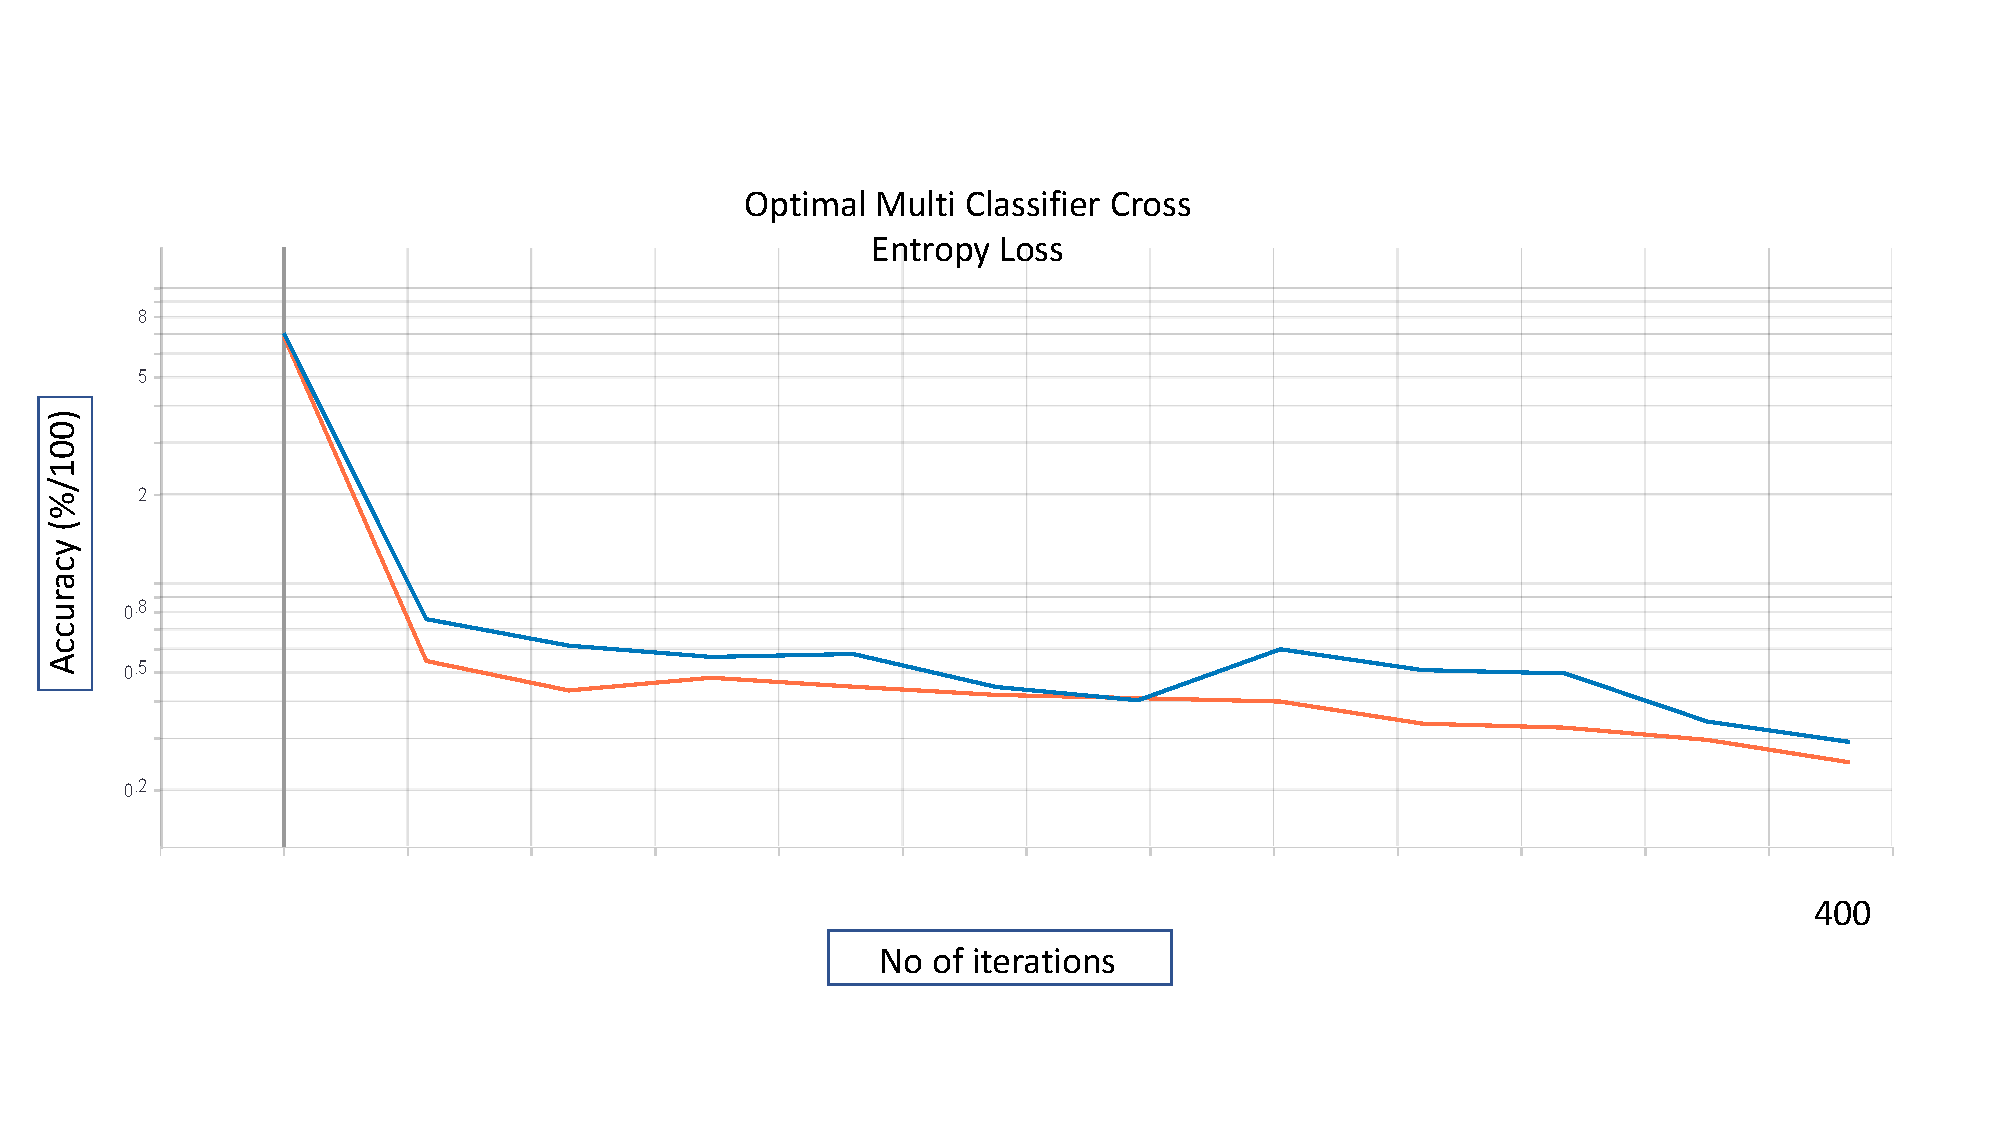
\includegraphics[width=1\textwidth]{../img/results/multiLoss.pdf}}
            \label{figX: Optimal Multi Loss Curves} 
            \caption{Optimal Multi Loss Curves; blue:training, orange:validation}
        \end{figure}
        
        For the training curve, both training and validation reach a high accuracy value hovering around 90\%, however it does not converge to a single value unlike what is seen in the binary classifier. The loss values for both curves do reach 0.25 competing with the binary classifier's performance. 
        
        \subsubsection{Inter-Observer Variability}
        The following are testing results when comparing the model against the 2 experts and one novice:
        \begin{figure}[h!]
            \centerline{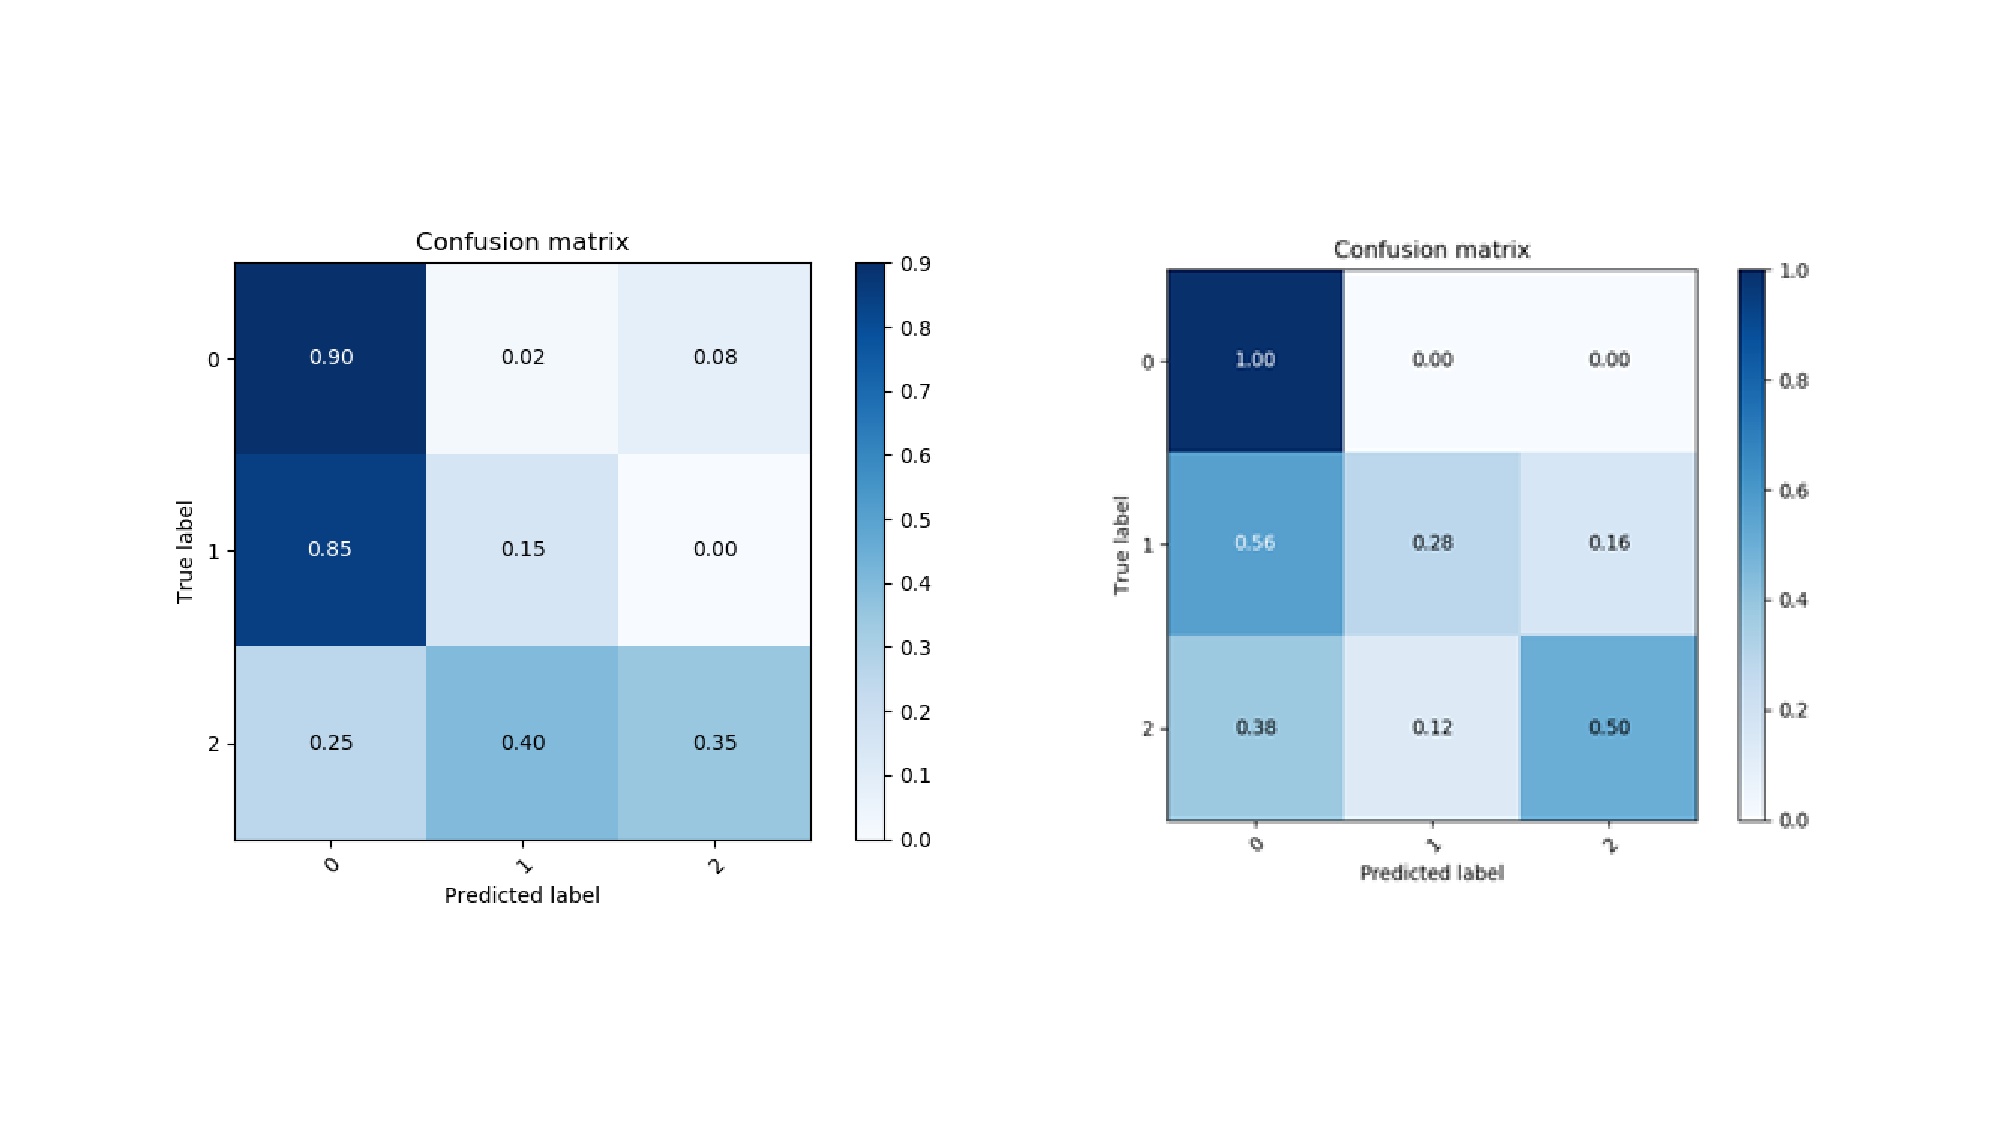
\includegraphics[width=1\textwidth]{../img/results/lisamichVsModel.pdf}}
            \label{figX: Model Vs Experts Confusion Matrix} 
            \caption{Model Vs Experts Confusion Matrix}
        \end{figure}
        \begin{figure}[h!]
            \centerline{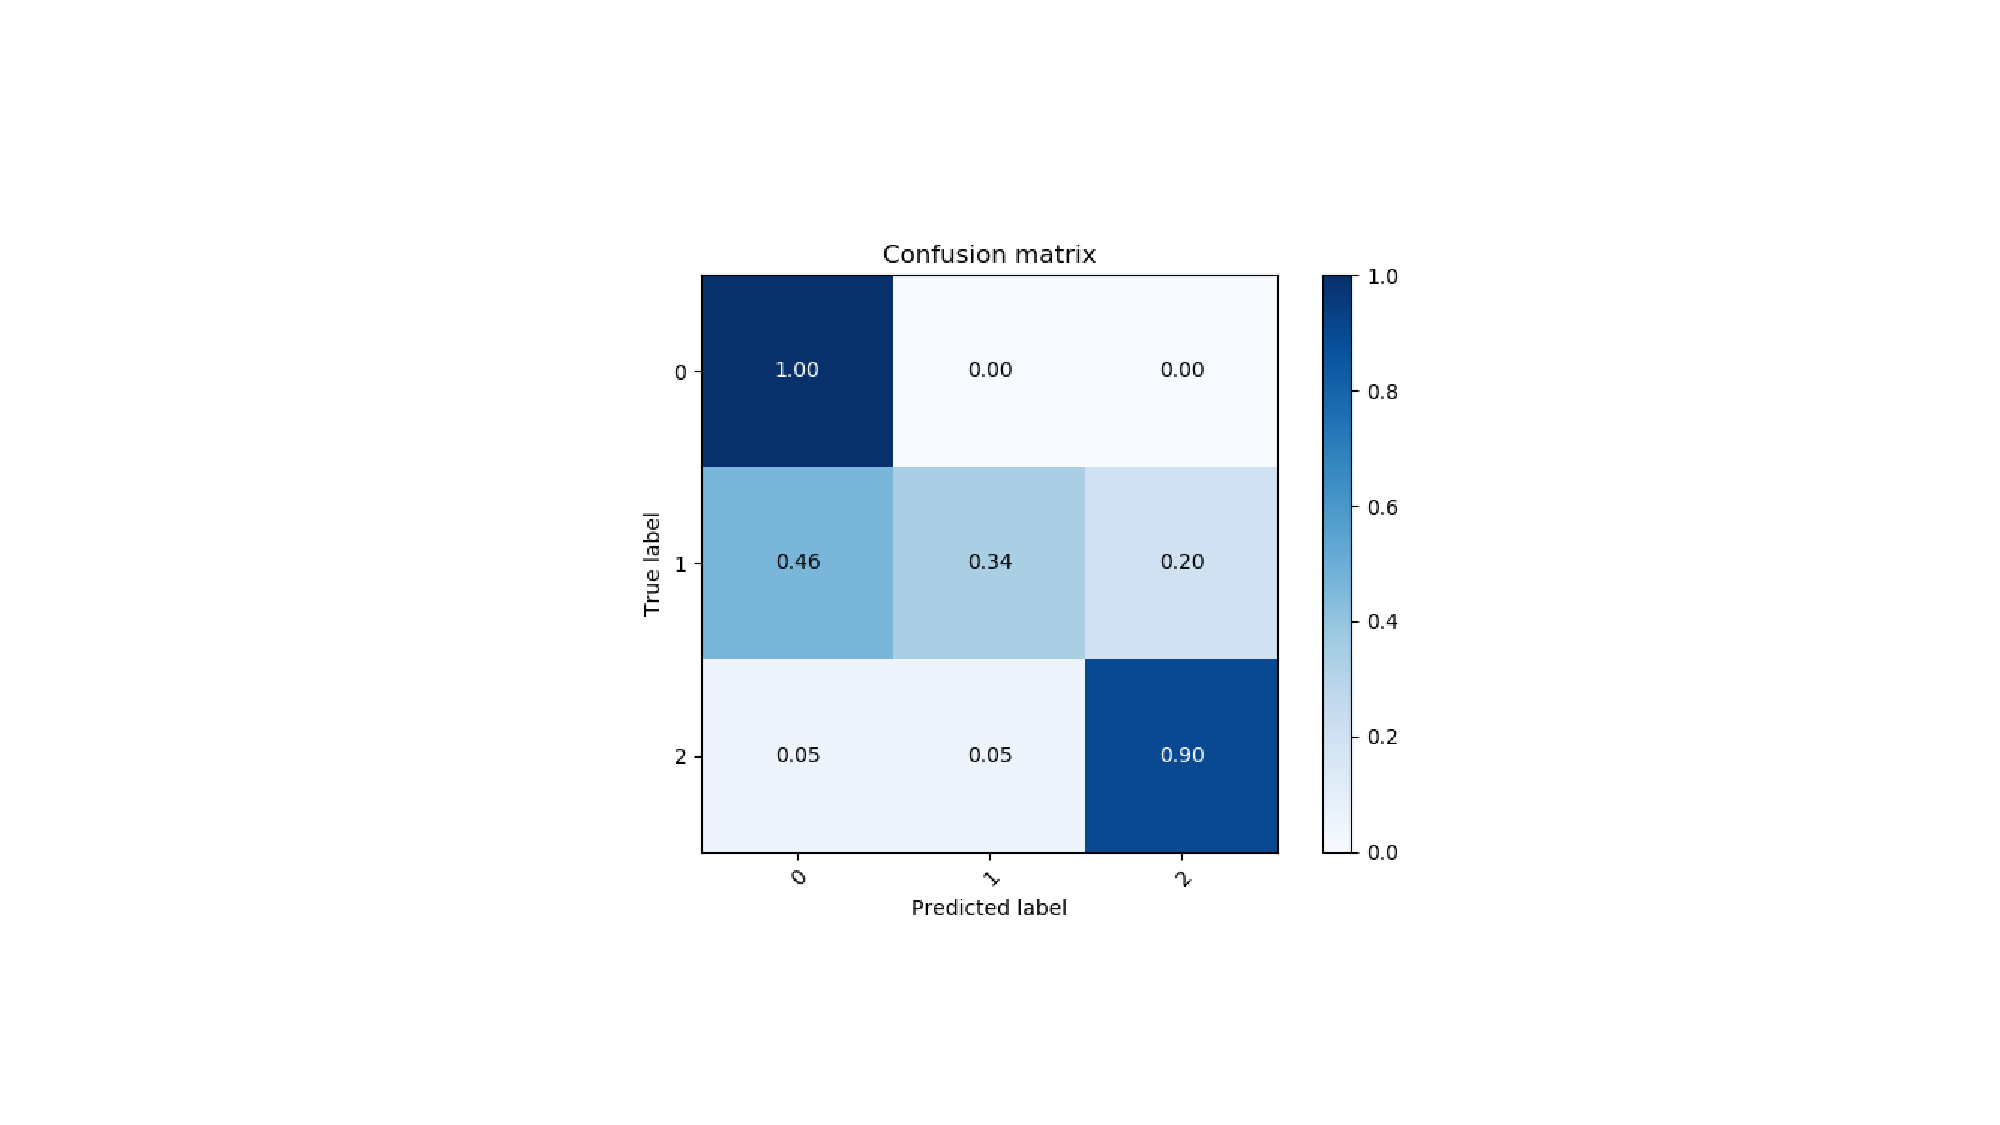
\includegraphics[width=1\textwidth]{../img/results/mohVsModel.pdf}}
            \label{figX: Model Vs Novice Confusion Matrix} 
            \caption{Model Vs Novice Confusion Matrix}
        \end{figure}

        It is very important to reiterate that both training and validation datasets were labelled by the novice (as discussed previously), only the testing datasets were labelled by the respectively observers who are included in the above confusion matrices. It measures the ratio of the model's predicted class over the true class labelled by that observer. All ratios in the same row sum up to 1.0 . It is clear that all observers agree with the model on the definition of a healthy retina. The model also agrees more with the novice's definition of a phase 2 as well. However, confusion arises when it comes to determining phases 1 for all observers and phase 2 for the experts.
        \vspace{3mm}

        Inter-observer variability tests between the experts were also conducted:
        \begin{figure}[h!]
            \centerline{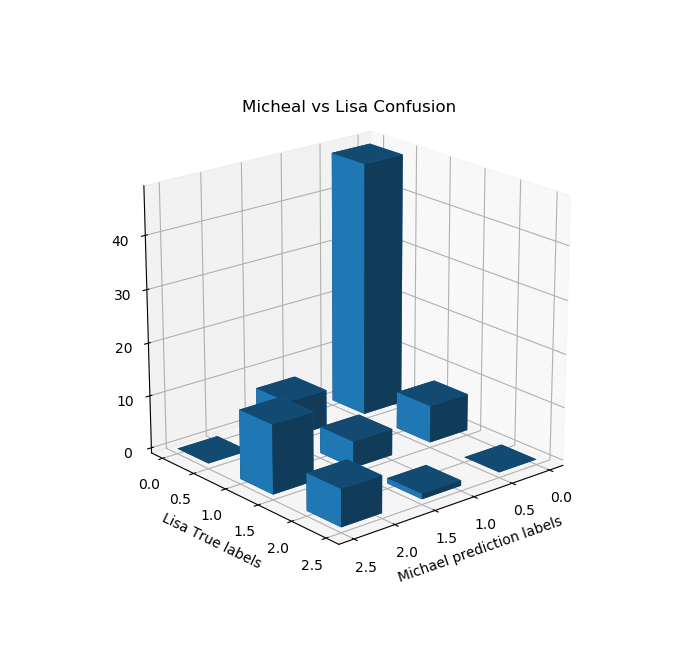
\includegraphics[width=0.5\textwidth]{../img/results/michVsLisa3d.PNG}}
            \label{figX: Expert Vs Expert Confusion Matrix} 
            \caption{Expert (Michael) Vs Expert (Lisa) Confusion Matrix}
        \end{figure}
        \begin{figure}[h!]
            \centerline{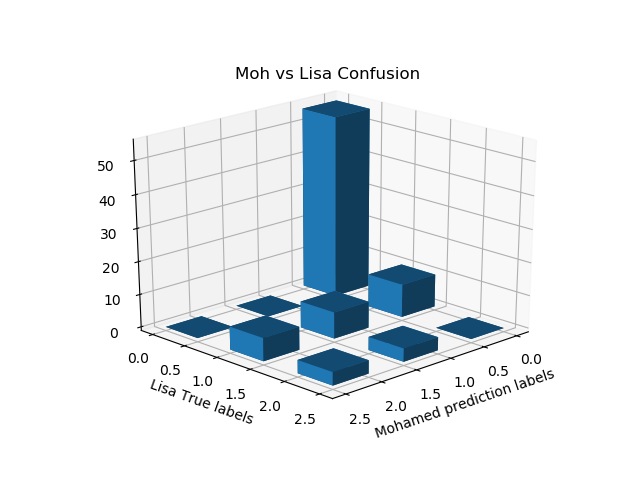
\includegraphics[width=0.5\textwidth]{../img/results/mohVsLisa3d.PNG}}
            \label{figX: Novice Vs Expert Confusion Matrix 1} 
            \caption{Novice (Mohamed) Vs Expert (Lisa) Confusion Matrix}
        \end{figure}
        \begin{figure}[h!]
            \centerline{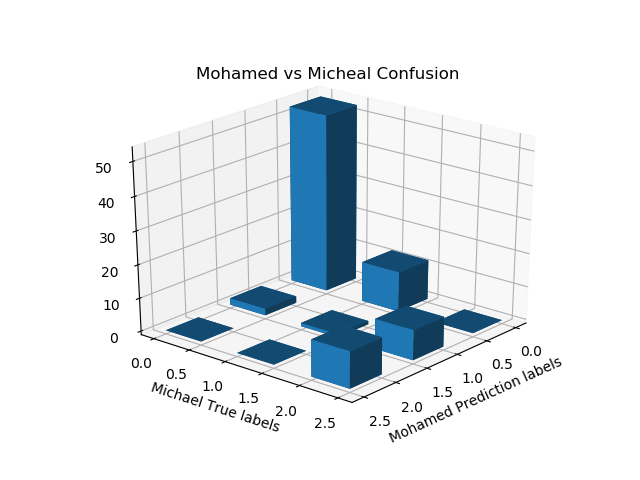
\includegraphics[width=0.5\textwidth]{../img/results/mohVsMich3d.PNG}}
            \label{figX: Model Vs Novice Confusion Matrix 2} 
            \caption{Novice (Mohamed) Vs Expert (Michael) Confusion Matrix}
        \end{figure}

        \newpage
        Each plot takes one of the observers as a reference, with an ideal plot showing "sky-scrappers" along the diagonal ((0, 0), (1, 1), (2, 2)). As expected, these plots mirror the previous results that all of the observers agree on phase 0 images with confusions about the remaining phases. A trend is evident, with the less-experienced expert (Lisa) tending to classify more images as phase 1, compared to the more-experienced expert who classified those images as phase 2. This is extended to the novice who tended to classify more images as phase 0 with a true label 1, and as phase 1 with a true label of 2 (against both experts). This supports the notion of "conservation level variation" between the observers. This will be discussed later on.
        \vspace{3mm}

        Results were also collected to analyse a 3-way classification of the different testing images show in the next 3 plots (the 3D plot was split into 3 smaller for easier visualisation for 2D representation):
        \begin{figure}[h!]
            \centerline{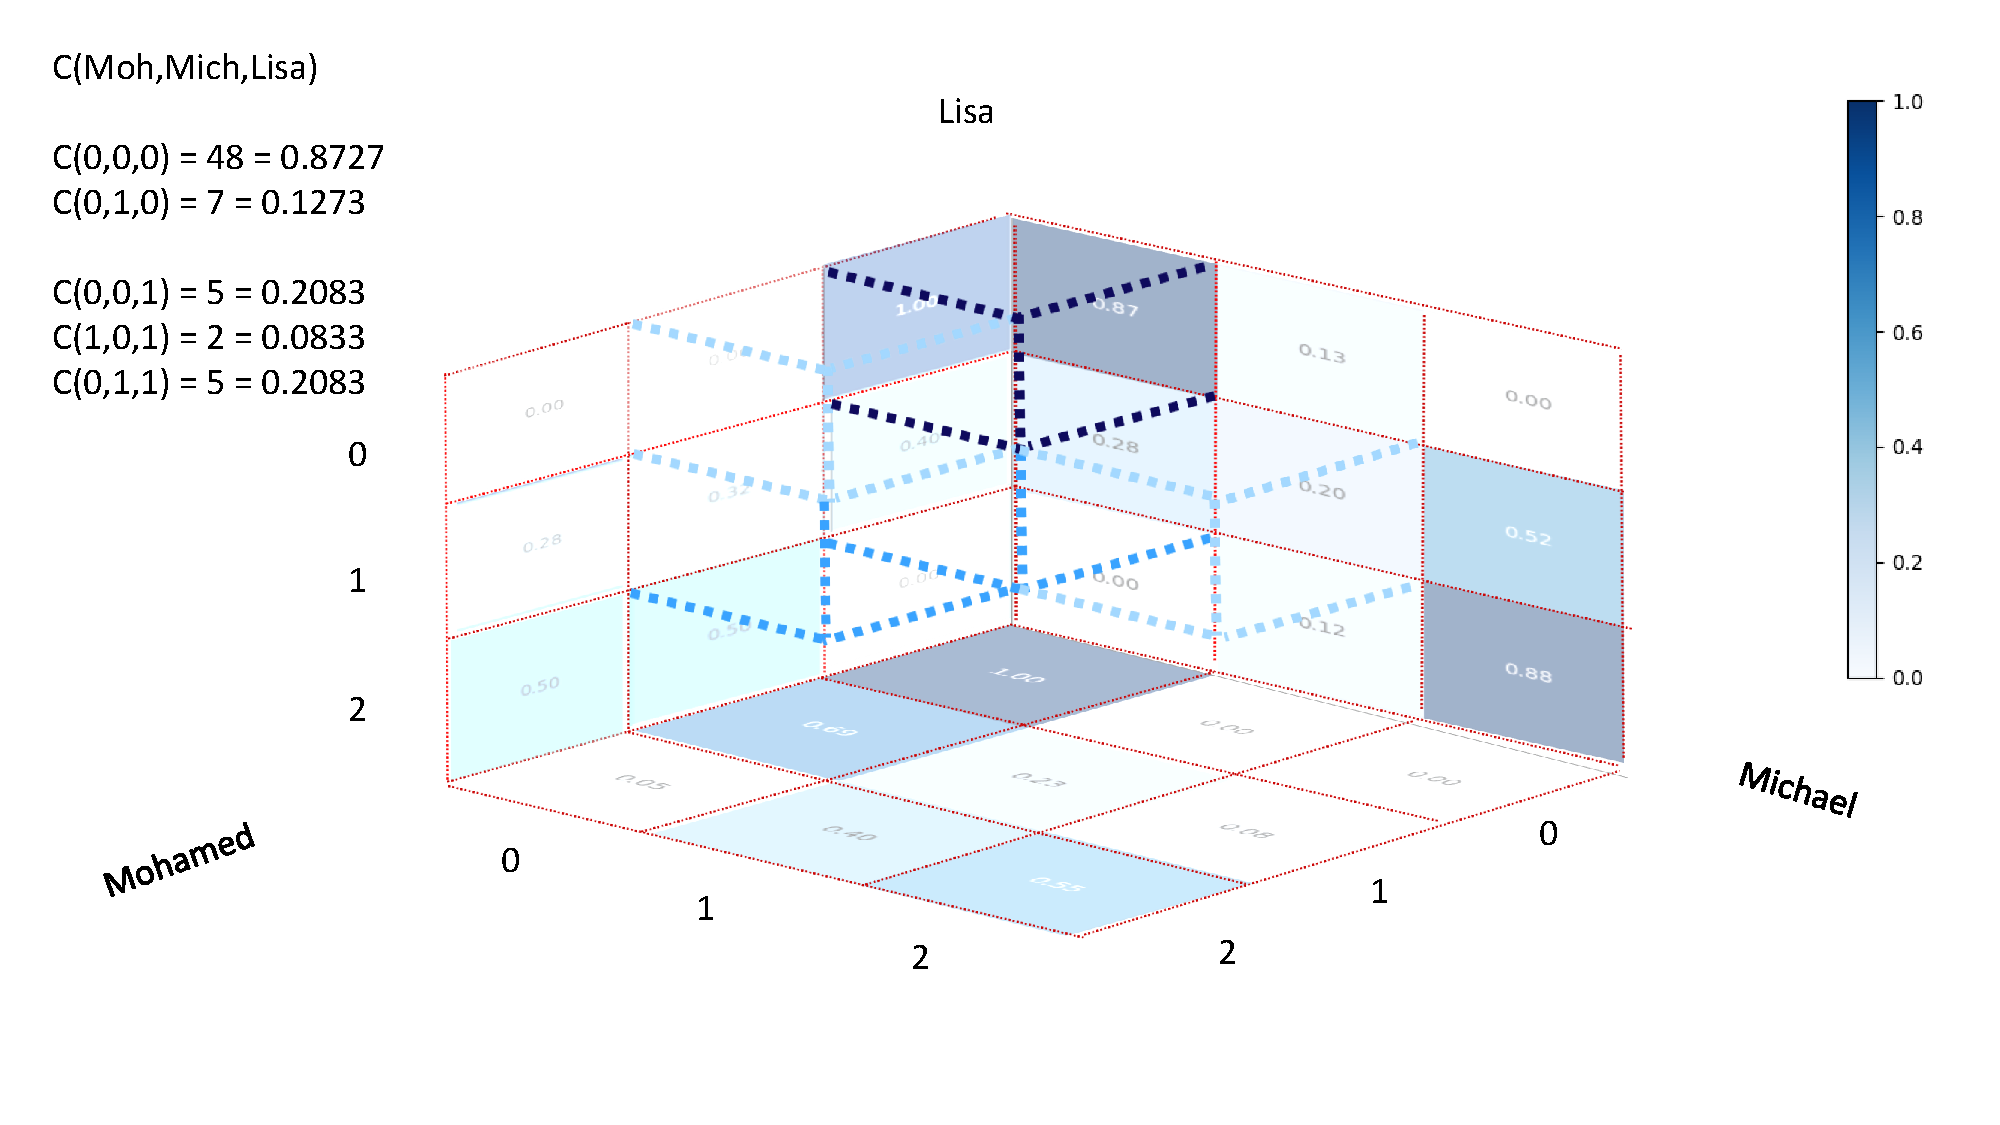
\includegraphics[width=0.5\textwidth]{../img/results/3dPlotPart1.pdf}}
            \label{figX: 3D Confusion Matrix (Part 1)} 
            \caption{3D Confusion Matrix; Novice(Mohamed) vs Expert(Michael) vs Expert(Lisa) (Part 1)}
        \end{figure}
        \begin{figure}[h!]
            \centerline{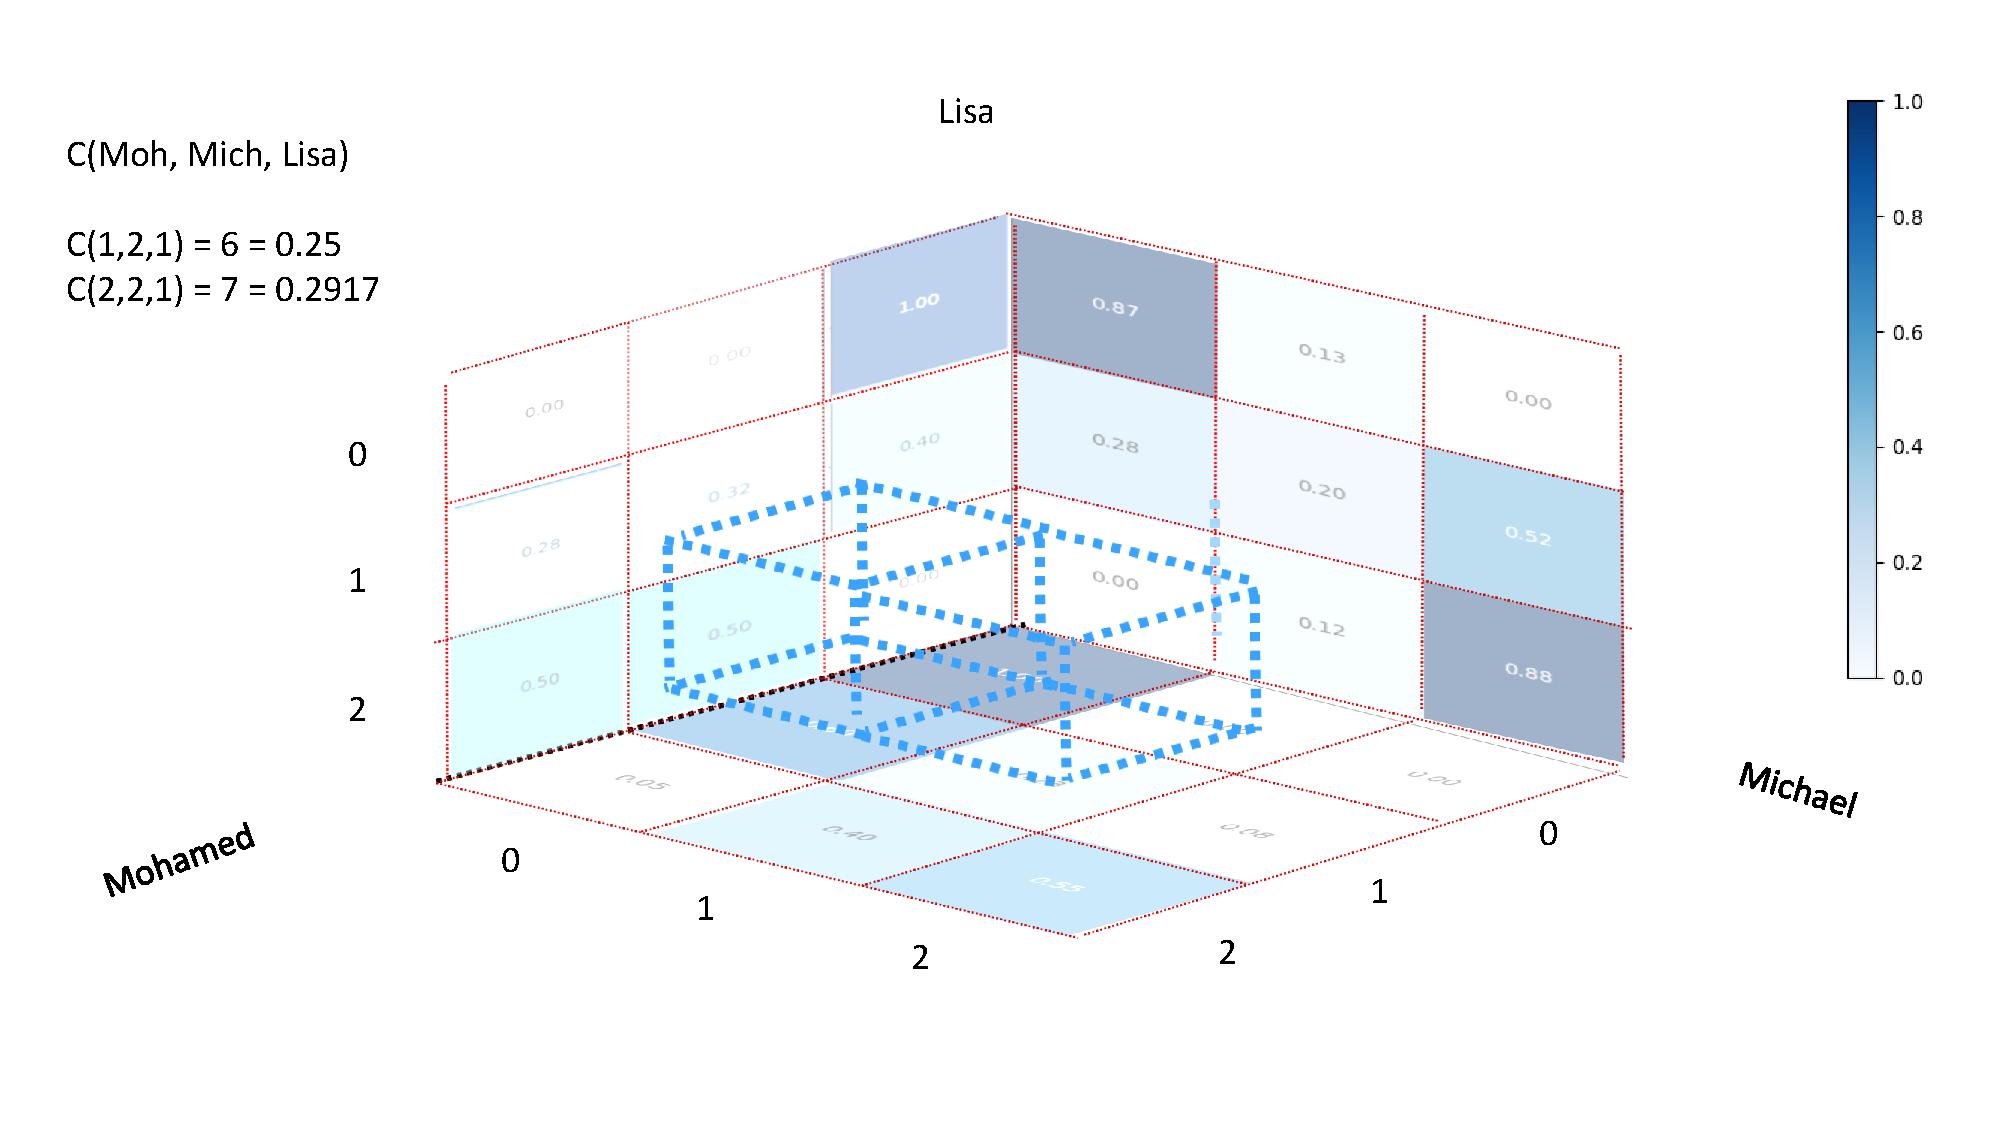
\includegraphics[width=0.5\textwidth]{../img/results/3dPlotPart2.pdf}}
            \label{figX: 3D Confusion Matrix (Part 2)} 
            \caption{3D Confusion Matrix; Novice(Mohamed) vs Expert(Michael) vs Expert(Lisa) (Part 2)}
        \end{figure}
        \begin{figure}[h!]
            \centerline{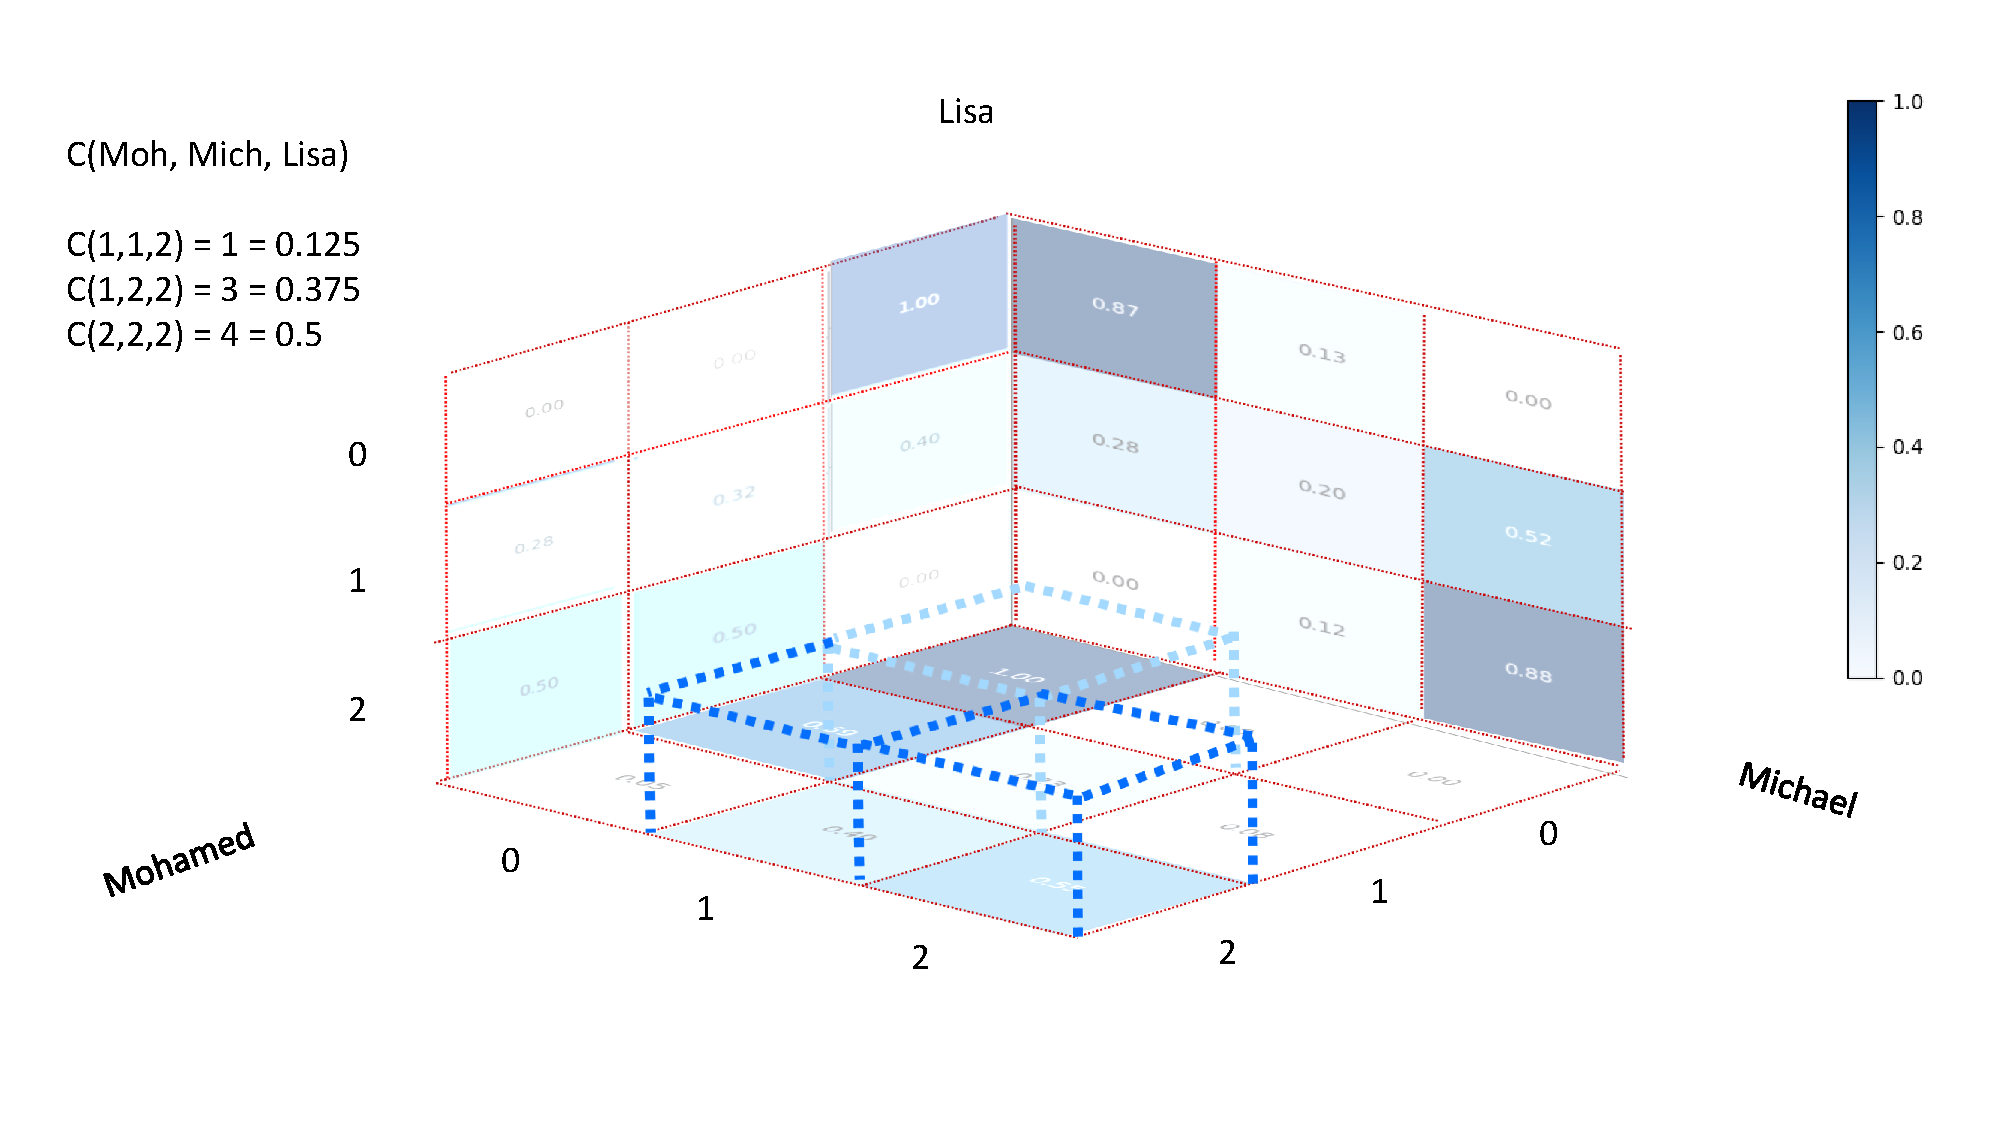
\includegraphics[width=0.5\textwidth]{../img/results/3dPlotPart3.pdf}}
            \label{figX: 3D Confusion Matrix (Part 3)} 
            \caption{3D Confusion Matrix; Novice(Mohamed) vs Expert(Michael) vs Expert(Lisa) (Part 3)}
        \end{figure}

\newpage
\section{Discussion}
    \subsection{Binary Classifier}
    The results obtained from this simple binary classifier were promising. It is clear that the criteria established to differentiate healthy retinae from damaged and/or blind ones are concise. The distinct boundary is evident in the validation accuracy which converges to around 88\% and the cross entropy log loss approaching 25\%, as well as high testing accuracy shown in table 8. The high accuracy suggests that a CNN is capable of identifying a well-processed set of images, labelled by an ophthalmology expert, into 2 clear categories (despite the training and validation sets being labelled by a novice). Modifications could have been made by allowing an expert to model the entire data to get a more concrete view of how a purely labelled set of data might perform. However, since this experiment is to establish whether AI has the ability to implemented in this type of histology, the current setup is sufficient to evaluate the claim.   
    \vspace{3mm}

    Considering that there is no publication or literature evidence to support the claim that such '\textit{Deep learning is capable of performing retinal classification using histological data}', this binary implementation is an encouraging step towards 'bridging-the-gap' in automated retinal analysis. Google's diabetic retinopathy classifier is an example of an AI that can base clinical predications on fundus photographs of the retina, basing its judgement solely on the analysis of the image only. The biological implications were extracted by the classifier when it began to develop its learning model (e.g. various blood vessels around the optic disc influence major cardiovascular factors that determine the formation of diabetes in a patient) from the type of images that it classified. Similarly, RetinaNETv0.1 was able to identify various biological factors within the retinal cellular structure that would influence why a certain image would portray a particular retina condition. The following images are examples that RetinaNETv0.1 would classify as healthy (first 2 images) and damaged/blind (last 2 images): 
    \begin{figure}[h!]
        \centerline{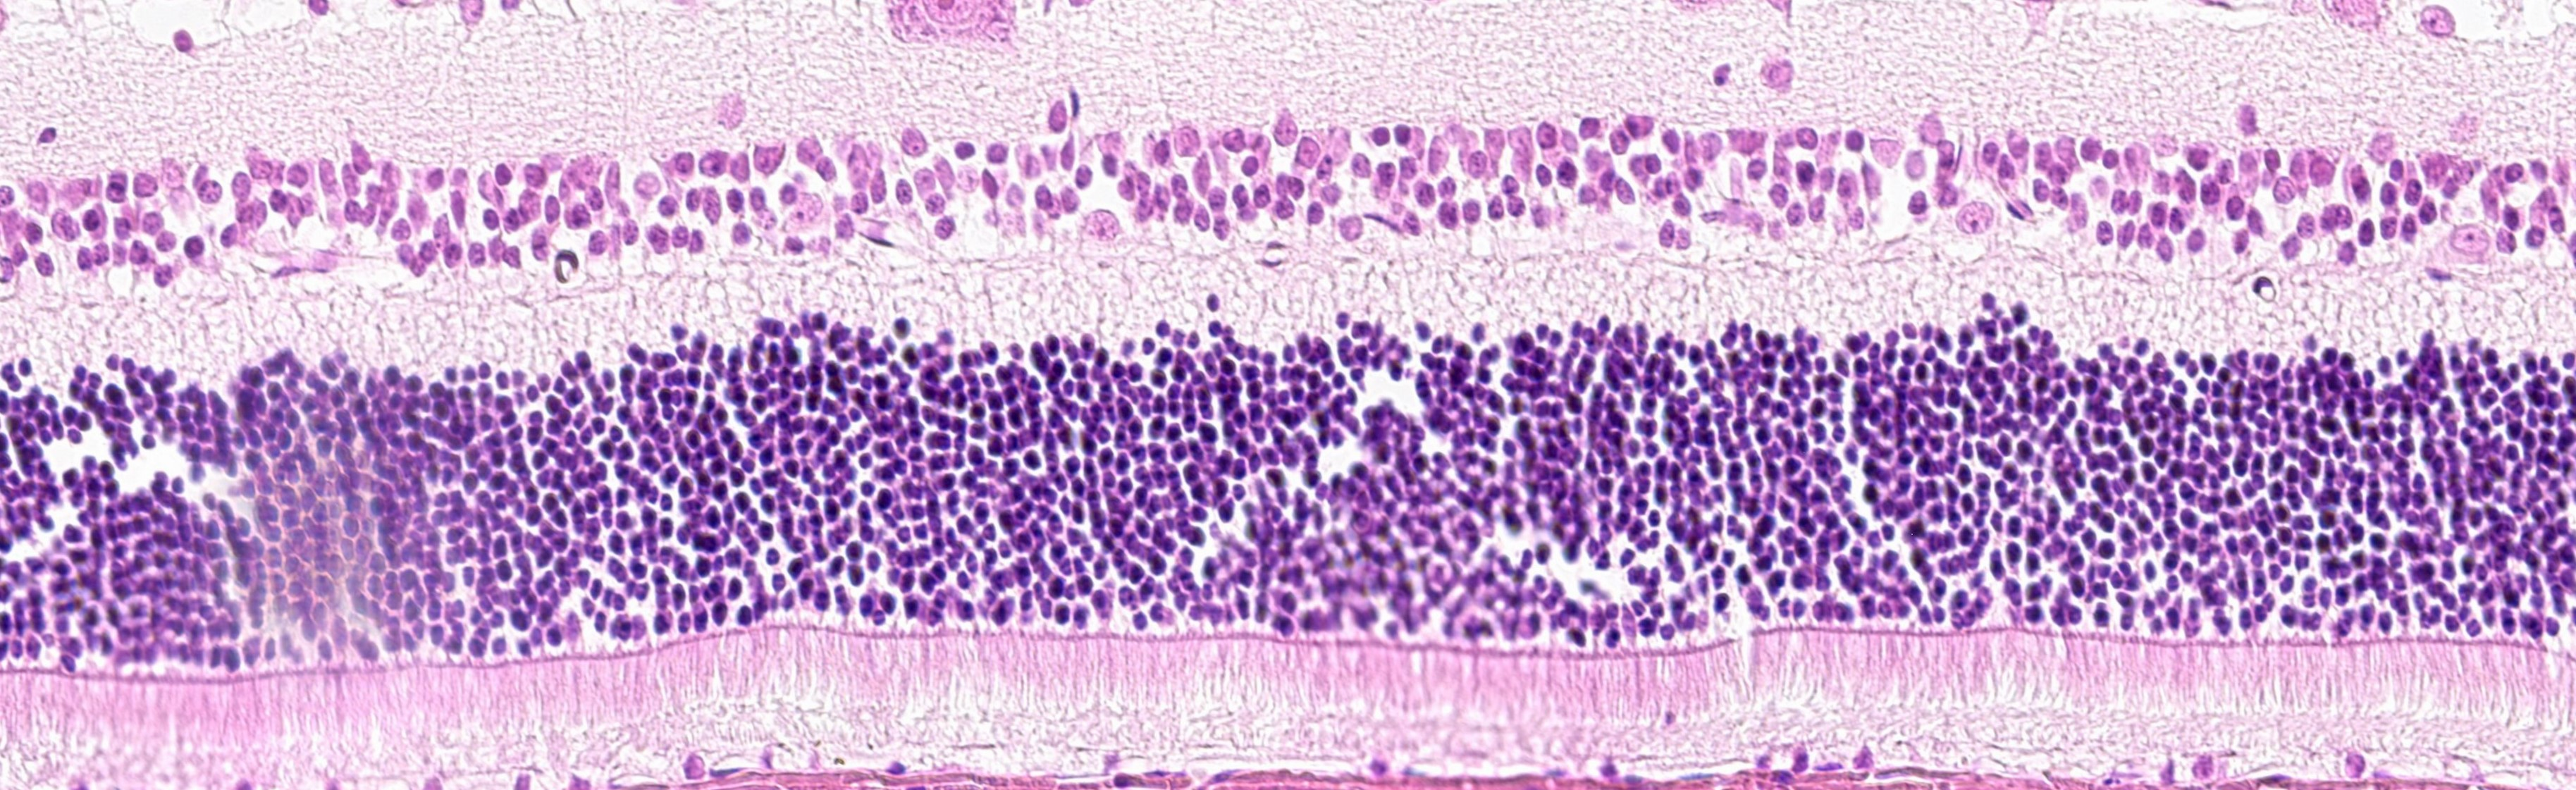
\includegraphics[width=0.5\textwidth]{../img/binary/normal1.jpg}}
        \centerline{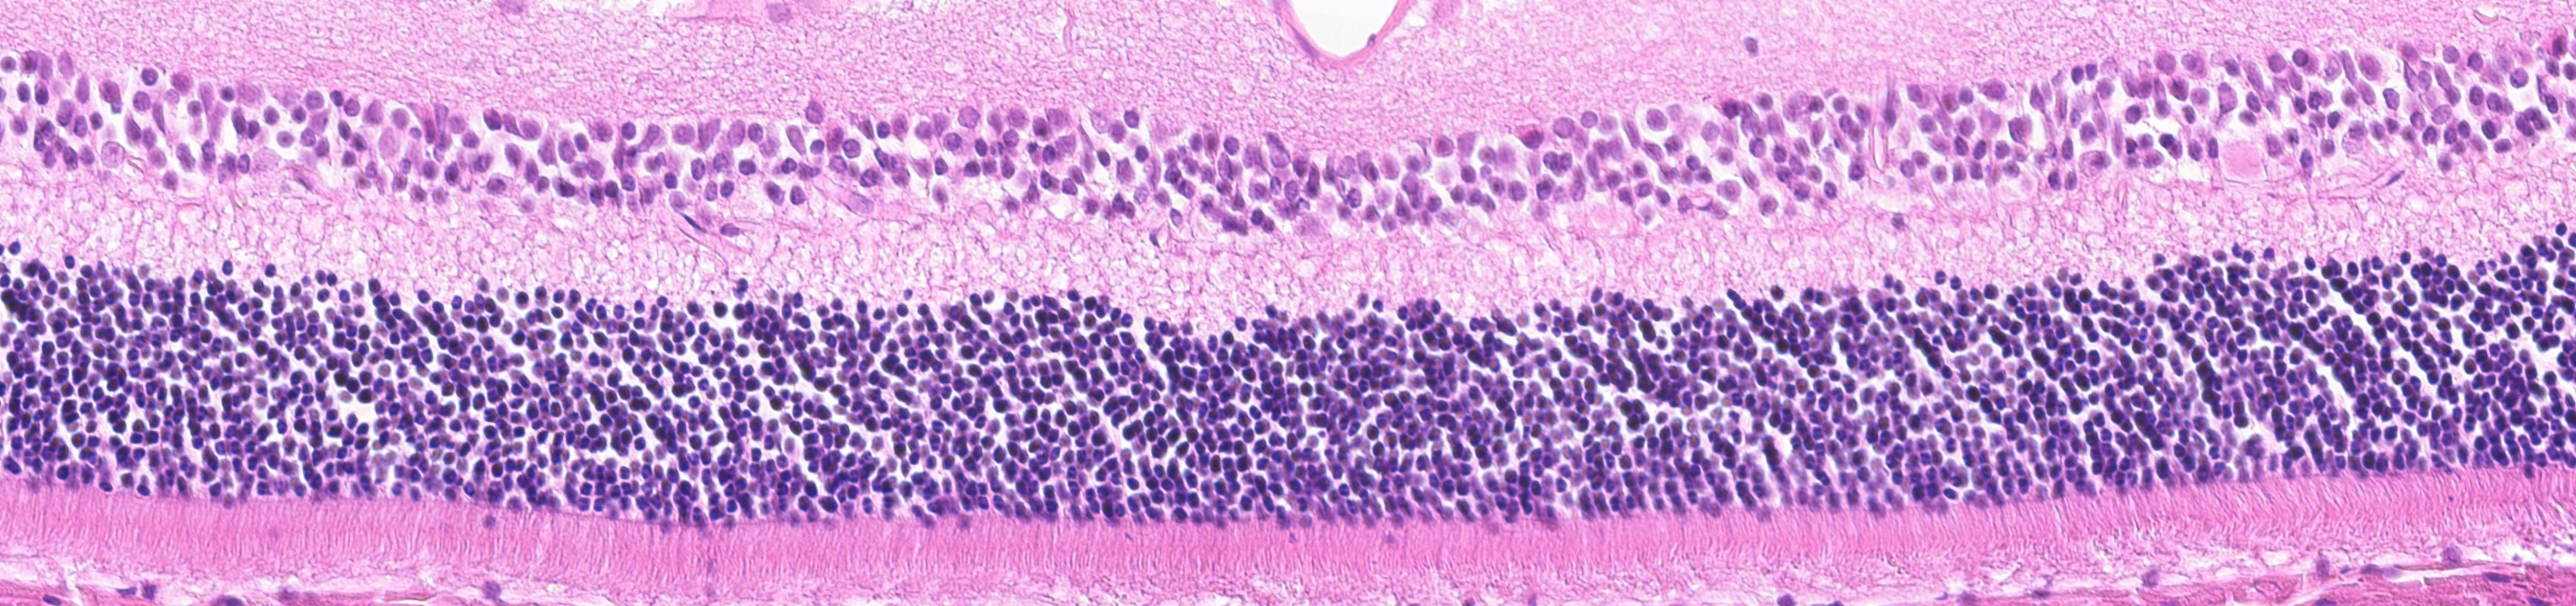
\includegraphics[width=0.5\textwidth]{../img/binary/normal2.jpg}}
        \vspace{3mm}
        \centerline{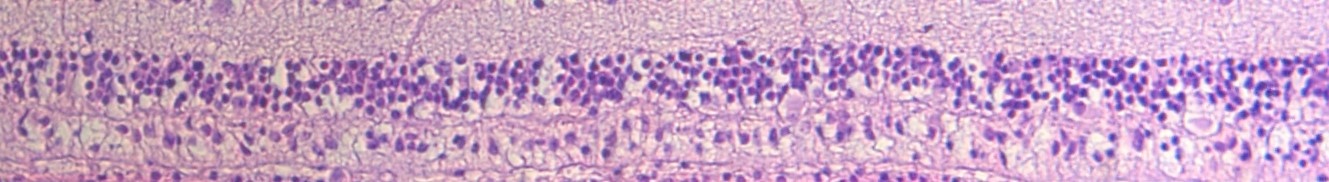
\includegraphics[width=0.5\textwidth]{../img/binary/blind1.jpg}}
        \centerline{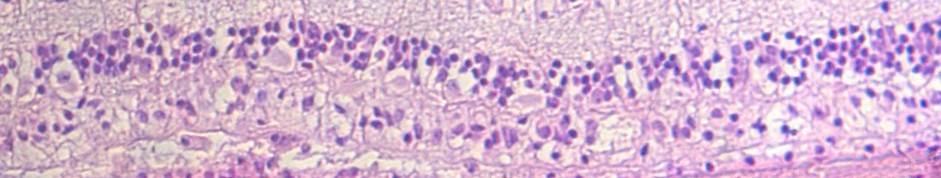
\includegraphics[width=0.5\textwidth]{../img/binary/blind2.jpg}}
    \end{figure}

    \vspace{3mm} 
    It is clear that the classifier is able to distinguish between the 2 classes based on biological factors, the same factors included in the blindness criteria discusses previously. Both nuclear layer densities are much lower in the blind class than in the healthy, in addition to the layers losing their smooth and laminar structure. Thus, the binary classifier experiment demonstrates the potential of AI in classification tasks that encompass retinal histology.
    
    \subsection{Multi Classifier}
    Confidence to develop a multi-classifier grew once it was established that an accurate and precise binary classifier is possible. Having said this, it was worthwhile conducting a full architecture search experiment to study architectural parameters that might affect a classifier's performance (particularly in biological applications). The exponential growth of AI (specifically deep learning) in such applications prompts the necessity to understand how a CNN architecture affects the performance. To this date, literature is unable to identify low-level factors that lead to a certain architecture's success or demise. 
    \vspace{3mm}

    The 2 architectural parameters chosen for this study were exclusively convolutional which affected the feature extraction from the images. Understanding how the number of inputs per convolutional layer affected this process is a key issue which literature is currently attempting to address. Additionally, the number of convolutional blocks in a CNN (usually referred to as the "Depth" of the convolution) is another intriguing factor to consider. 
    \vspace{3mm}

    Interestingly, the experiment conducted in this project was able to locate a specific architecture that outperformed the rest (that were tested). The solution lays not at one of the extreme cases of both parameters (e.g. 1 block + (16,32), 3 blocks + (64,128)), but somewhat near the middle of the search space. The optimal solution did not require the maximum number of outputs per layer but did require 3 levels of convolutional blocks. It was the best solution among the 8 other architectures, but continued to face issues with images from the mildly-damaged class. The accuracy and log loss values were the best for this specific model as was its weighted F1 score. An important trend that can be established here is the tendency of the model to classify images with damage that ranges from very minimal to just below blinding as a healthy retina. Due to the model's minimal experience in classifying such images, it preferred to remain less conservative when prompting to classify low-damaged retinae. As will be discussed in the inter-observer variability, the notion of "conservation level variation" begins to appear in the model's performance and is extended to the other observers results. 
    \vspace{3mm}

    As for the training and validation for this optimal architecture, accuracy converged to around 90\% and loss was able to reduce to lower than 30\%. These indicate that the model could have been improved after 400 epochs, and further training and validation could have remedied the poor class-1 classification. 
    \vspace{3mm}

    The unbalanced number of samples for each class shown in table 6 did not affect the performance according to the confusion matrix. Despite more images being labelled as class 1 by a considerable margin, the model struggled to identify testing images labelled as this class which it had not seen previously (during training or validation). This resulted in a weighted F1 score of 82\% for this architecture. Other architectural factors may have helped improved the ability to classify this class more accurately, for example the implementation of dropout on the convolutions. This would randomly "deactivate" neurons in the layers and assist the model improve performance on this class.
    \vspace{3mm}

    \begin{figure}[h!]
        \centerline{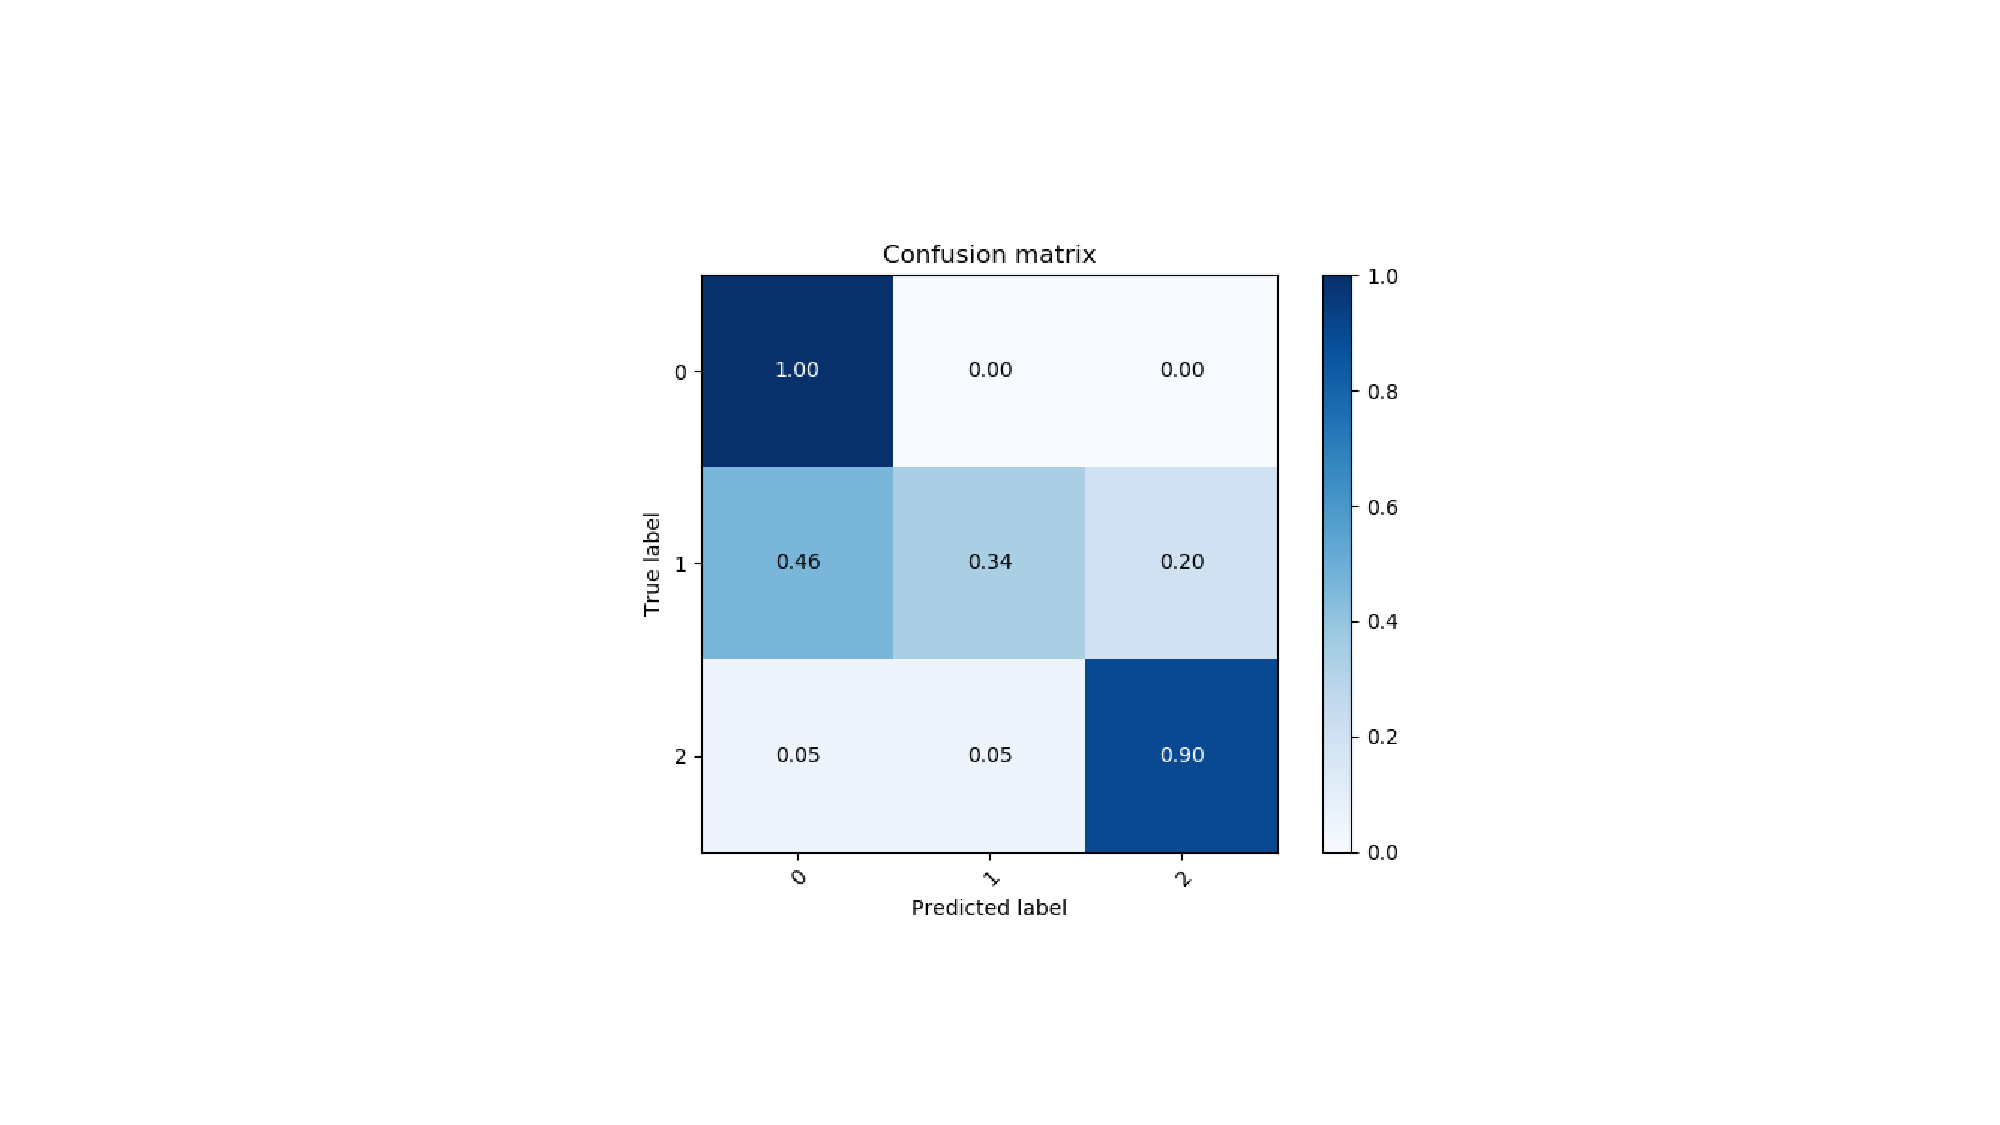
\includegraphics[width=1.2\textwidth]{../img/results/mohVsModel.pdf}}
    \end{figure}

    It is also worthwhile to analyse the architecture's superiority to the others and establish why it was able to outperform them. Table 6 shows a significant decrease in model performance when the complexity is increased, in both dimensions. the exception arose with the $(Conv_{11}(64) \rightarrow Conv_{12}(128)) \Rightarrow (Conv_{21}(64) \rightarrow Conv_{22}(128))$ case. It is interesting to see that the (16,32) and (32,64) showed similar decreases in performance when increasing the number of convolutional blocks. The model would begin to overfit once its complexity grew too large, suggesting that the less complex the model was, the better it would perform on this type of data.

    \subsection{Inter Observer Variability}
    It can be observed that the 3 observers (2 experts, novice) along with the optimal multi classifier architecture face no difficulties when attempting to define a healthy retina structure. Astonishingly, Figure 11 shows that the model tended to be less conservative, once again. The model would only determine an image to be a representation of mild or significant damage if very clear signs of damage were present. The notion of "conservation level variation" appears in the variability between the model and experts, suggesting that the model's experience is inversely proportional to its estimation of damage conversation. The modelling tends to be less conservative with its definition of retinal damage and blindness. These are samples of images labelled as mildly-damaged (class 1) by expert Michael (first 2) and expert Lisa (last 2):
    \begin{figure}[h!]
        \centerline{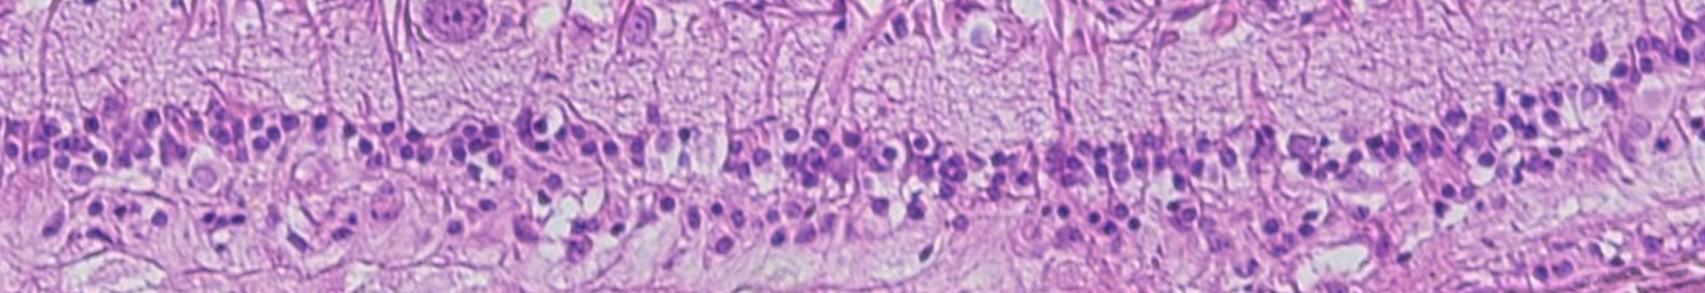
\includegraphics[width=0.5\textwidth]{../img/multi/lisa11.jpg}}
        \centerline{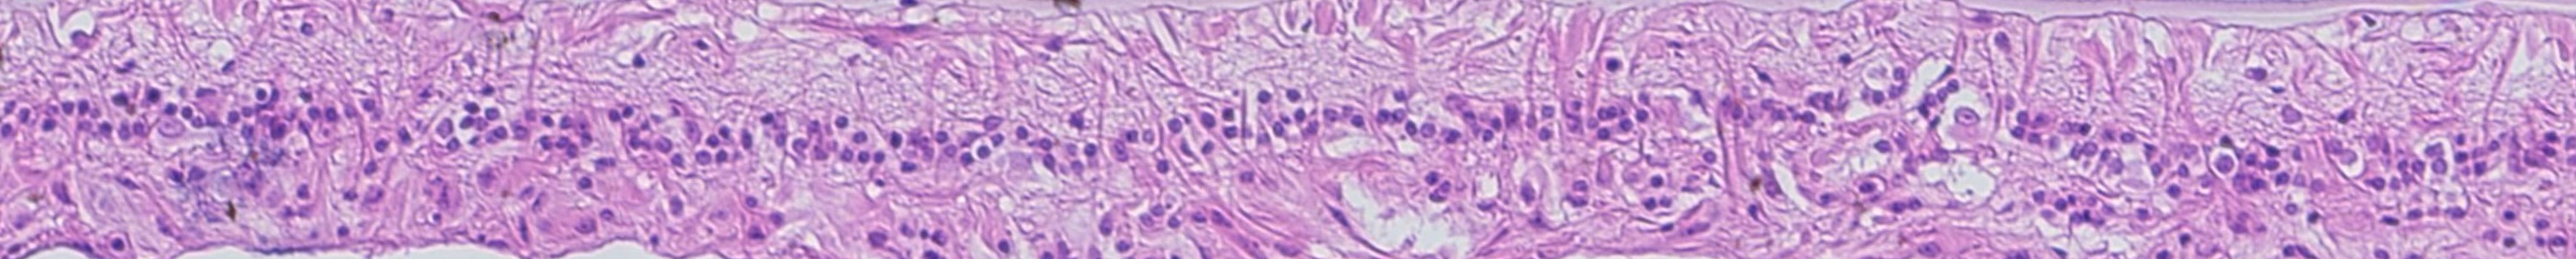
\includegraphics[width=0.5\textwidth]{../img/multi/lisa12.jpg}}
        \vspace{3mm}
        \centerline{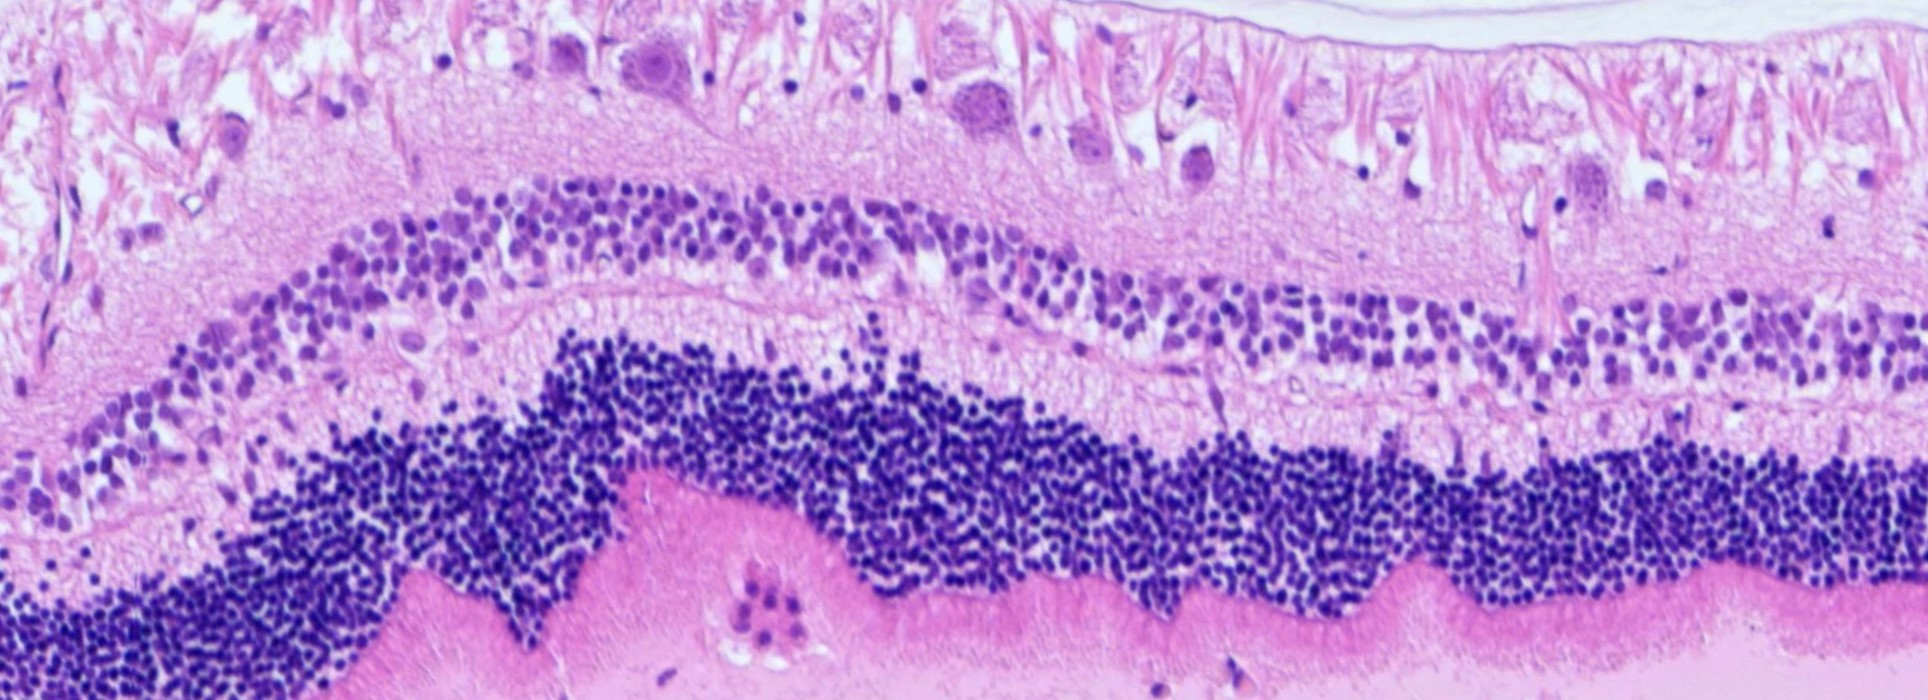
\includegraphics[width=0.5\textwidth]{../img/multi/mich11.jpg}}
        \centerline{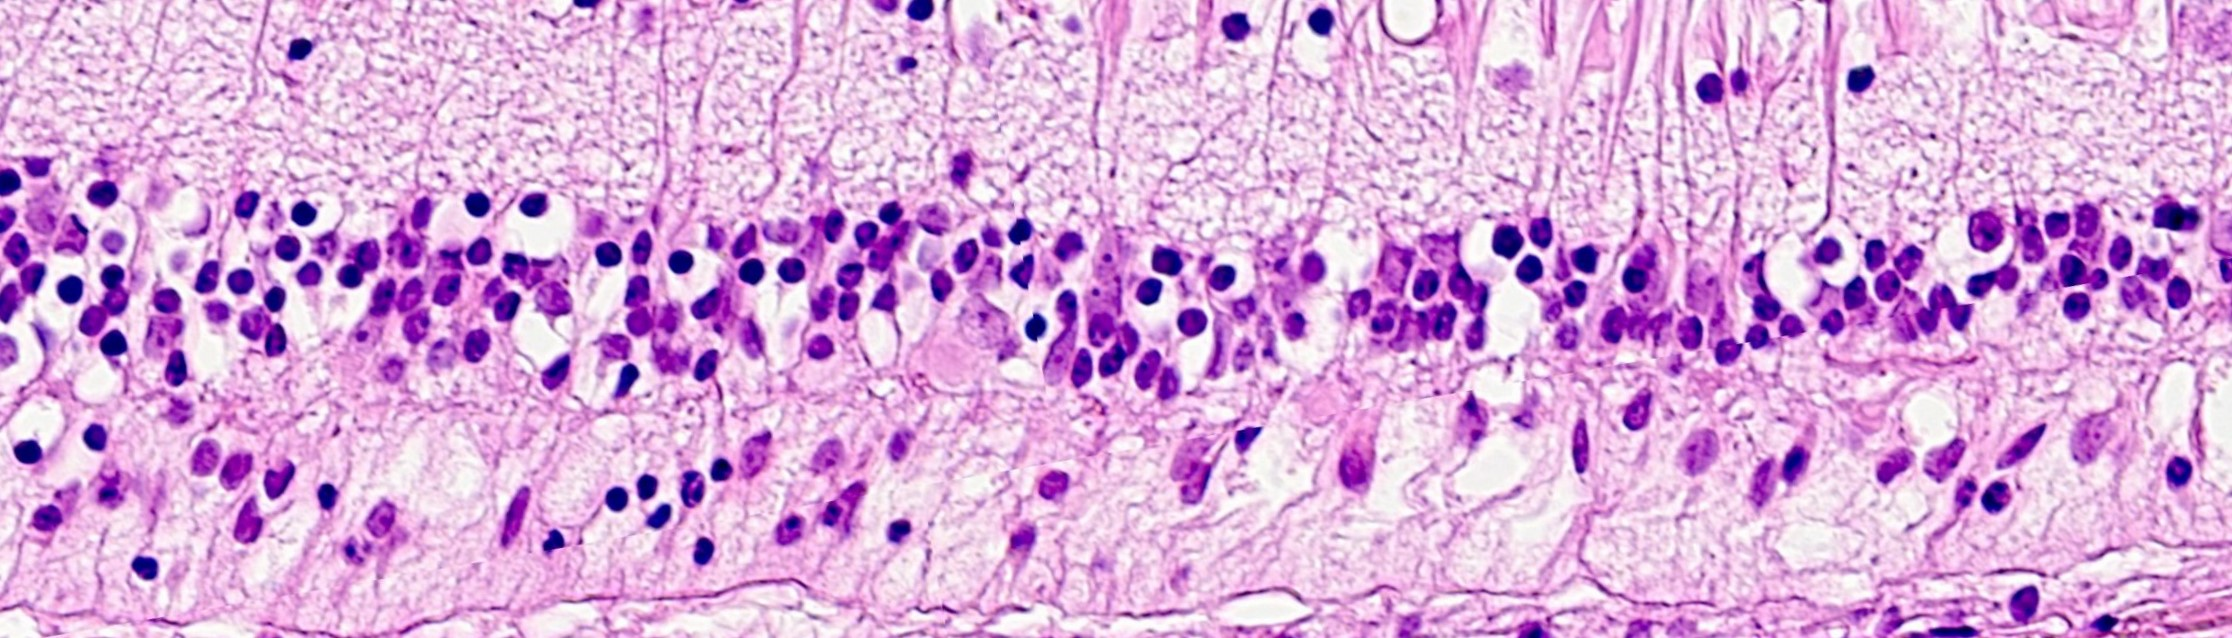
\includegraphics[width=0.5\textwidth]{../img/multi/mich12.jpg}}
    \end{figure}
    \vspace{3mm}

    However, this notion can be extended to the inter observer variability tests as well. Figure 13 demonstrates that both experts have various ideas of what constitutes as mildly damaged and completely blind. Furthermore, expert "Lisa" tended to be less conservative than expert "Michael". For example, the 2 experts have different experiences in retinal classification with "Michael" being in this field for a longer period of time than "Lisa". Having stated this, both observers' level of experience seem to be inversely proportional with the damage conservation estimation level.  

    \noindent\rule{17cm}{0.4pt}
    \begin{center}
        \textbf{{\huge $e(x) \propto \frac{1}{c(x)}$ }}\\
    \end{center}
    where:
    \vspace{3mm}
    
    \textbf{e(x)}: experience of expert x
    \vspace{3mm}
    
    \textbf{c(x)}: damage conservation estimation of expert x.\\
    \noindent\rule{17cm}{0.4pt}
    \vspace{3mm}

    Ultimately, when comparing the model's performance to the novice and experts, it clear that it follows this trend of conservation variation. Due to the novice labelling all training and validation datasets, the model will resemble the novice in classification and either be on par or worse than the novice.  
    
    \noindent\rule{17cm}{0.4pt}
    \begin{center}
        \textbf{{\huge $p(model) \leq p(novice) < p (experts)$ }}\\
    \end{center}
    where:
    \vspace{3mm}

    \textbf{p(x)}: performance of observer x\\
    \noindent\rule{17cm}{0.4pt}
    \vspace{3mm}

    Finally, a reassuring aspect of this study is the fact that all 3 observers have not resorted to 3 different definitions for a single class. Figures16-18 show that there is no case where an image classified by Lisa as class 0 is classified by Michael as class 1 and Mohamed as class 2. This goes for all 3 different combinations of a 3-way classification of an testing image. Once more, the confusion only lies when attempting to define distinct boundaries between the damage classes (1-2).     


    \subsection{Future plans for RetinaNET} 
    RetinaNET shows the potential of applying AI to retinal histological data, as it was able to produce a well-defined binary classifier. This itself is a great step towards the parameterisation of blindness on a cellular level. The achievement to universally agree on the definition of a \textbf{healthy retinal structure} is a stepping-stone towards building a more solid foundation in retinal degeneration analysis. More meaningful classifications will depend on this binary classifier as a precursor when defining the blindness criteria. 
    \vspace{3mm}
    
    As discussed previously, no 2 experts, when given no appropriate context to the set problem, agree on the definitions of retinal damage classes. Thus a classifier must be able to capture different interpretations of retinal damage from experts. Approaches to labelling the training and validation datasets must be refined in a way that will allow for a full-proof  capture of features. Several experts may label these datasets prior to developing the model and could provide a more consistent classifier that resembles experts in the real-world. However, this approach will still contain flaws as the confusion between the experts themselves will produce contradictions in the model's interpretation of the features. 
    \vspace{3mm}

    From a computer science perspective, the CNNs have performed well on both classification criteria (binary/multi). The confusion that arises from the labelling of the data can also be addressed by developing an unsupervised model. This approach will give the model an opportunity to extract hidden, biological features from images that may not be clear to any expert. This may be the best future step towards building a better classifier, as it will not rely on the uncertainties of experts and will depend on:
    \begin{itemize}
        \item the architecture's ability to extract features that will segregate images into different classes.
        \item appropriate normalisation and pre-processing of the datasets.
    \end{itemize}        
    \vspace{3mm}

\newpage
\section{Conclusion}
In conclusion, the attempted implementation of a binary classifier for H\&E stained images was successful, demonstrating that it is able to identify clearly damaged from healthy retina. The multi classifier requires refinement from an architectural and class criteria perspective. Both classifiers are clear indications of AI's potential and will no doubt be beneficial for future studies of retinal degeneration and its practical solutions. The foundation to retinal histological analysis using deep learning has been established and future studies in this field should address the issues that affected this study. Once a reliable model which earns the experts' trust is ready, the preparation of a mathematical model that parameterises blindness on a histological level will be the final step. The findings of this project are encouraging to the degree that such a feat in automated retinal degeneration analysis is accomplishable.


\pagebreak
\bibliography{thesis}
\bibliographystyle{ieeetr}

\section{Acknowledgements}
    \begin{itemize}
        \item \textbf{Prof Michael Kalloniatis}, School of Optometry and Vision Science-UNSW: Ophthalmology expert.
        \item \textbf{Dr Lisa Nivison-Smith}, School of Optometry and Vision Science-UNSW: Ophthalmology expert.
        \item \textbf{Prof Erik Meijering}, Graduate School of Biomedical Engineering-UNSW: Project Co-supervisor.
        \item \textbf{Dr Mohit Shivdasani}, Graduate School of Biomedical Engineering-UNSW: Project supervisor.   
    \end{itemize}
\section{Appendix}
    \begin{itemize}
        \item Hyperparameters chosen for all classifiers:
            \begin{itemize}
                \item Optimizer: ADAM
                \item Learning Rate: 0.001
                \item Loss function: SoftMax Cross-Entropy with logits
                \item Batch size: 32
                \item Training/Validation split: 70-30
                \item Number of Epochs: 400
            \end{itemize}
        \item GitHub Repository containing the different models produced for this project: \\
                \textbf{https://github.com/M-Almouie/thesis} 
        \item Google Drive link containing the datasets of H\&E stained retina images:\\
                \textbf{https://drive.google.com/drive/folders/1-6s-smvnVkUF5qkK0AEnUstOy2QXFQUN?usp=sharing}
    \end{itemize}
\end{document}